\selectlanguage{english}

The force of gravity is mediated by a gravitational field, which is identified with a metric $ g_{\mu \nu}(x) $ on a 4d Lorentzian manifold called spacetime. This metric is a dynamical object, as all other fields in Nature, thus the laws governing its dynamics must be studied.

\section{Einstein-Hilbert action}

Differential Geometry places strict limits to the possible actions that can be formulated, ensuring it is something intrinsic to the metric and independent on the particular choice of coordinates.\\
Spacetime is a Lorentzian manifold $ \mathcal{M} $, thus, recalling the canonical volume form in Eq. \ref{eq:3.13}, there need to be metric-dependent scalar function on $ \mathcal{M} $: the obvious non-trivial choice is the Ricci scalar. The resulting action is the \textit{Einstein-Hilbert action}:
\begin{equation}
  \mathcal{S} = \int d^4 x \sqgm R
  \label{eq:4.1}
\end{equation}
where the negative sign makes it manifest that the metric has signature $ (-,+,+,+) $. Schematically, the Riemann tensor is $ R \sim \pa \Gamma + \Gamma \Gamma $, while $ \Gamma \sim \pa g $, thus the Einstein-Hilbert action is second order in derivatives of the metric, like most other actions in physics.

\subsection{Equations of motion}

To determine the Euler-Lagrange equations of the Einstein-Hilbert action, consider a fixed initial metric $ g_{\mu \nu}(x) $ and a perturbation $ g_{\mu \nu}(x) \mapsto g_{\mu \nu}(x) + \delta g_{\mu \nu}(x) $. For the inverse metric:
\begin{equation*}
  g_{\mu \nu} g^{\nu \rho} = \delta_\mu^\rho
  \quad \Rightarrow \quad
  \delta g_{\mu \nu} g^{\nu \rho} + g_{\mu \nu} \delta g^{\nu \rho} = 0
  \quad \Rightarrow \quad
  \delta g^{\mu \nu} = - g^{\mu \rho} g^{\nu \sigma} \delta g_{\rho \sigma}
\end{equation*}

\begin{lemma}\label{lemma-sqgm}
  The variation of $ \sqgm $ is:
  \begin{equation}
    \delta \sqgm = - \frac{1}{2} \sqgm\, g_{\mu \nu} \delta g^{\mu \nu}
    \label{eq:4.2}
  \end{equation}
\end{lemma}
\begin{proof}
  Recalling that for a diagonalizable matrix $ \log \det A = \tr \log A $, then $ (\det A)^{-1} \delta (\det A) = \tr (A^{-1} \delta A) $. Applying this to the metric:
  \begin{equation*}
    \delta \sqgm = \frac{1}{2} \frac{1}{\sqgm} \delta (-\tens{g}) = \frac{1}{2} \frac{1}{\sqgm} (-\tens{g}) g^{\mu \nu} \delta g_{\mu \nu} = \frac{1}{2} \sqgm\, g^{\mu \nu} \delta g_{\mu \nu} = - \frac{1}{2} \sqgm\, g_{\mu \nu} g^{\mu \nu}
  \end{equation*}
\end{proof}

\begin{lemma}
  The variation of the Christoffel symbols is:
  \begin{equation}
    \delta \Gamma^\rho_{\mu \nu} = \frac{1}{2} g^{\rho \sigma} ( \na_\mu \delta g_{\sigma \nu} + \na_\nu \delta g_{\sigma \mu} - \na_\sigma \delta g_{\mu \nu} )
    \label{eq:4.3}
  \end{equation}
\end{lemma}
\begin{proof}
  First note that, although $ \Gamma^\rho_{\mu \nu} $ is not a tensor, $ \delta \Gamma^\rho_{\mu \nu} $ is, for it is the difference of two Christoffel symbols, one computed with $ g_{\mu \nu} $ and the other with $ g_{\mu \nu} + \delta g_{\mu \nu} $, but the extra term in the transformation law of $ \Gamma^\rho_{\mu \nu} $ is independent of the metric, thus cancels out.\\
  This osservation allows to work in normal coordinates at $ p \in \mathcal{M} $, so that $ \pa_\rho g_{\mu \nu} = 0 $ and $ \Gamma^\rho_{\mu \nu} = 0 $ at that point. Then, to linear order in the variation, at $ p $:
  \begin{equation*}
    \delta \Gamma^\rho_{\mu \nu} = \frac{1}{2} g^{\rho \sigma} ( \pa_\mu \delta g_{\sigma \nu} + \pa_\nu \delta g_{\sigma \mu} - \pa_\sigma \delta g_{\mu \nu} ) = \frac{1}{2} g^{\rho \sigma} ( \na_\mu \delta g_{\sigma \nu} + \na_\nu \delta g_{\sigma \mu} - \na_\sigma \delta g_{\mu \nu} )
  \end{equation*}
  This is a tensor equation, hence valid in all coordinate system and, being $ p $ arbitrary, on all $ \mathcal{M} $.
\end{proof}

\begin{lemma}
  The variation of the Ricci tensor is:
  \begin{equation}
    \delta R_{\mu \nu} = \na_\rho \delta \Gamma^\rho_{\rho \nu} - \na_\nu \delta \Gamma^\rho_{\rho \mu}
    \label{eq:4.4}
  \end{equation}
\end{lemma}
\begin{proof}
  Working in normal coordinates, the Riemann tensor becomes $ \tensor{R}{^\sigma_{\mu \rho \nu}} = \pa_\rho \Gamma^\sigma_{\nu \mu} - \pa_\nu \Gamma^\sigma_{\rho \mu} $, so:
  \begin{equation*}
    \delta \tensor{R}{^\sigma_{\mu \rho \nu}} = \pa_\rho \delta \Gamma^\sigma_{\nu \mu} - \pa_\nu \delta \Gamma^\sigma_{\rho \mu} = \na_\rho \delta \Gamma^\sigma_{\nu \mu} - \na_\nu \delta \Gamma^\sigma_{\rho \mu}
  \end{equation*}
  This is a tensor equation, hence valid in all coordinates systems and on all $ \mathcal{M} $. Contracting indices $ \sigma,\rho $ and working to leading order yields the result.
\end{proof}

\begin{proposition}\label{prop-einst-eq}
  The Euler-Lagrange equations of the Einstein-Hilbert action are:
  \begin{equation}
    G_{\mu \nu} = 0
    \label{eq:4.5}
  \end{equation}
\end{proposition}
\begin{proof}
  Varying the Einstein-Hilbert action:
  \begin{equation*}
    \begin{split}
      \delta \mathcal{S}
      &= \delta \int d^4 x \sqgm\, g^{\mu \nu} R_{\mu \nu} \\
      &= \int d^4 x \left[ \delta (\sqgm) g^{\mu \nu} R_{\mu \nu} + \sqgm (\delta g^{\mu \nu}) R_{\mu \nu} + \sqgm\, g^{\mu \nu} (\delta R_{\mu \nu}) \right] \\
      &= \int d^4 x \sqgm \left[ \left( - \frac{1}{2} R g_{\mu \nu} + R_{\mu \nu} \right) \delta g^{\mu \nu} + g^{\mu \nu} \left( \na_\rho \delta \Gamma^\rho_{\mu \nu} - \na_\nu \Gamma^\rho_{\rho \mu} \right) \right] \\
      &= \int d^4 x \sqgm \left[ \left( R_{\mu \nu} - \frac{1}{2} R g_{\mu \nu} \right) \delta g^{\mu \nu} + \na_\mu \left( g^{\rho \nu} \nu \Gamma^\mu_{\rho \nu} - g^{\mu \nu} \delta \Gamma^\rho_{\rho \nu} \right) \right]
    \end{split}
  \end{equation*}
  The last term is a total derivative, hence by the divergence theorem Eq. \ref{eq:3.41} it yields a boundary term which can be ignored (Gibbons-Hawking boundary term). The Euler-Lagrange equations are then found imposing $ \delta \mathcal{S} $ for arbitrary $ \delta g_{\mu \nu} $, so recalling the definition of the Einstein tensor Eq. \ref{eq:3.66} the proof is completed.
\end{proof}

These equations are called \textit{Einstein field equations} in the absence of any matter. For this reason, they can be further simplified: by contracting with $ g^{\mu \nu} $ one finds $ R = 0 $, thus:
\begin{equation}
  R_{\mu \nu} = 0
  \label{eq:4.6}
\end{equation}

\subsubsection{Dimensional analysis}

The Einstein-Hilbert action in Eq. \ref{eq:4.1} doesn't have the right dimensions, which will be necessary when considering the presence of matter.\\
If $ x^\mu $ has dimension of length, then $ g_{\mu \nu} $ is dimensionless and the Ricci scalar is $ [R] = L^{-2} $. Including the integration measure $ [\mathcal{S}] = L^2 $, but it must have the same dimension of $ [\hbar] =  M L^2 T^{-1} $ (i.e. energy $ \times $ times). Thus, the action with the right dimension is:
\begin{equation}
  \mathcal{S} = \frac{c^3}{16 \pi G} \int d^4 x \sqgm R
  \label{eq:4.7}
\end{equation}
In the following, natural units are adopted: $ c = \hbar = 1 $.

\subsubsection{Cosmological constant}

It reality, Eq. \ref{eq:4.1} is not the simplest action allowed by Differential Geometry: in fact, a constant term could be added to the Ricci scalar. The action then becomes:
\begin{equation}
  \mathcal{S} = \frac{1}{16 \alpha G} \int d^4 x \sqgm (R - 2 \Lambda)
  \label{eq:4.8}
\end{equation}
$ \Lambda $ is called the \textit{cosmological constant} and has dimension $ [\Lambda] = L^{-2} $. The resulting field equations are:
\begin{equation}
  R_{\mu \nu} - \frac{1}{2} R g_{\mu \nu} = - \Lambda g_{\mu \nu}
  \label{eq:4.9}
\end{equation}
Contracting with $ g^{\mu \nu} $ yields $ R = 4\Lambda $, thus in the absence of matter:
\begin{equation}
  R_{\mu \nu} = \Lambda g_{\mu \nu}
  \label{eq:4.10}
\end{equation}

\subsection{Diffeomorphisms}

Being the metric a symmetric $ \R^{4,4} $ matrix, it should have $ \frac{1}{2} \times 4 \times 5 = 10 $ degrees of freedom. However, not all the components of $ g_{\mu \nu} $ are physical. Indeed, two metrics related by a change of coordinates $ x^\mu \mapsto \tilde{x}^\mu(x) $ describe the same physical spacetime, thus there is a redundancy in any given representation of the metric, which removes precisely 4 degrees of freedom, leaving with only 6 remaining degrees of freedom.\\
Mathematically, given a diffeomorphism $ \phi : \mathcal{M} \rightarrow \mathcal{M} $, it maps all fields on $ \mathcal{M} $ to a new set of fields on $ \mathcal{M} $: the result is physically indistinguishable from the original, describing the same spacetime but in different coordinates. Such diffeomorphisms are analogous to gauge symmetries in Yang-Mills theory.\\
Consider a diffeomorphism $ x^\mu \mapsto \tilde{x}^\mu = x^\mu + \delta x^\mu $: this can be viewed as an active change, where points in spacetime are mapped from one another, or as a passive change, in which only the coordinates of each point are affected, but the two are equivalent. This change of coordinates can be thought as generated by an infinitesimal vector field $ X^\mu : \delta x^\mu = - X^\mu (x) $, so that the metric transforms as:
\begin{equation*}
  \begin{split}
    \tilde{g}_{\mu \nu} (\tilde{x})
    &= \frac{\pa x^\rho}{\pa \tilde{x}^\mu} \frac{\pa x^\sigma}{\pa \tilde{x}^\nu} g_{\rho \sigma}(x) = \left( \delta^\rho_\mu + \pa_\mu X^\rho \right) \left( \delta^\sigma_\nu + \pa_\nu X^\sigma \right) g_{\rho \sigma}(x) \\
    &= g_{\mu \nu}(x) + g_{\mu \rho}(x) \pa_\nu X^\rho + g_{\nu \rho}(x) \pa_\mu X^\rho
  \end{split}
\end{equation*}
Meanwhile, the Taylor expansion around $ \tilde{x} = x + \delta x $ is:
\begin{equation*}
  \tilde{g}_{\mu \nu} (\tilde{x}) = \tilde{g}_{\mu \nu} (x + \delta x) = \tilde{g}_{\mu \nu}(x) - X^\lambda \pa_\lambda \tilde{g}_{\mu \nu}(x)
\end{equation*}
Comparing the metrics at the same point, it is understood that it undergoes an infinitesimal change:
\begin{equation*}
  \delta g_{\mu \nu}(x) = \tilde{g}_{\mu \nu}(x) - g_{\mu \nu}(x) = X^\lambda \pa_\lambda g_{\mu \nu}(x) + g_{\mu \rho}(x) \pa_\nu X^\rho + g_{\nu \rho}(x) \pa_\mu X^\rho
\end{equation*}
By Eq. \ref{eq:2.23}, this is the Lie derivative of the metric:
\begin{equation}
  \delta g_{\mu \nu} = (\ld_X g)_{\mu \nu}
  \label{eq:4.11}
\end{equation}
Thus, an infinitesimal diffeomorphism along $ X \in \xm $ makes the metric change by an infinitesimal amount given by its Lie derivative along $ X $. This can be viewed as the leading term in the Taylor expansion along $ X $. These equations can be rewritten in a simpler form:
\begin{equation*}
  \delta g_{\mu \nu} = X^\rho \pa_\rho g_{\mu \nu} + \pa_\nu X_\mu - X^\rho \pa_\nu g_{\mu \rho} + \pa_\mu X_\nu - X^\rho \pa_\mu g_{\nu \rho} = \pa_\mu X_\nu + \pa_\nu X_\mu + 2 g_{\rho \sigma} \Gamma^\sigma_{\mu \nu} X^\rho
\end{equation*}
Therefore:
\begin{equation}
  \delta g_{\mu \nu} = \na_\mu X_\nu + \na_\nu X_\mu
  \label{eq:4.12}
\end{equation}
This equation can be used in the path integral. In fact, insisting that $ \delta \mathcal{S} = 0 $ for any $ \delta g_{\mu \nu} $ gives the equations of motion; on the other hand, those variations $ \delta g_{\mu \nu} $ for which $ \delta \mathcal{S} = 0 $ for any metric are the \textit{symmetries} of the action. From Prop. \ref{prop-einst-eq}:
\begin{equation*}
  \delta \mathcal{S} = \int d^4 x \sqgm\, G^{\mu \nu} \delta g_{\mu \nu} = 2 \int d^4 x \sqgm\, G^{\mu \nu} \na_\mu X_\nu
\end{equation*}
Invariance for $ x^\mu \mapsto x^\mu - X^\mu $ means that $ \delta \mathcal{S} = 0 $ for all $ X \in \xm $, hence, integrating by parts:
\begin{equation}
  \na_\mu G^{\mu \nu} = 0
  \label{eq:4.13}
\end{equation}
This is Bianchi identity: although it is a result from Differential Geometry, is follows from diffeomorphism invariance of the Einstein-Hilbert action. Bianchi identity is comprised of 4 equations, which make the 10 Einstein equations not completely independent: in fact, only 6 of then are independent, the same number of independent components of the metric, thus ensuring that the field equations are not overdetermined.

\section{Simple solutions}

The Einstein equations in the absence of matter are:
\begin{equation*}
  R_{\mu \nu} = \Lambda g_{\mu \nu}
\end{equation*}
with $ \Lambda \in \R $.

\subsection{Minkowski space}

The simplest case is $ \Lambda = 0 $. The Einstein equations then reduce to $ R_{\mu \nu} = 0 $, with the condition of $ g_{\mu \nu} $ being non-degenerate, for it is a metric and the field equations require the existence of the inverse metric $ g^{\mu \nu} $. This restriction is physically unusual: it is not a holonomic constraint on the physical degrees of freedom, but an inequality $ \det g < 0 $ (with required signature $ (-,+,+,+) $) which is not found for other fields of the Standard Model.\\
The simplest Ricci flat metric is Minkowski space $ ds^2 = -dt^2 + d\ve{x}^2 $, but it is not the only metric obeying $ R_{\mu \nu} = 0 $. Another example is Schwarzschild metric.

\subsection{de Sitter space}

Consider $ \Lambda > 0 $. A possible ansatz is:
\begin{equation*}
  ds^2 = - f(r)^2 dt^2 + f(r)^{-2} dr^2 + r^2 (d\vartheta^2 + \sin^2 \vartheta d\varphi^2)
\end{equation*}

\subsubsection{Riemann tensor}

First, one needs to compute the Ricci tensor for this metric: a simple way is using the curvature form. The non-coordinate 1-forms satisfy $ d^2 = \eta_{ab} \hat{\theta}^a \otimes \hat{\theta}^b $, thus:
\begin{equation*}
  \hat{\theta}^0 = f dt
  \qquad
  \hat{\theta}^1 = f^{-1} dr
  \qquad
  \hat{\theta}^2 = r d\vartheta
  \qquad
  \hat{\theta}^3 = r \sin \vartheta d\varphi
\end{equation*}
\begin{equation*}
  d\hat{\theta}^0 = f' dr \wedge dt
  \qquad
  d\hat{\theta}^1 = 0
  \qquad
  d\hat{\theta}^2 = dr \wedge d\vartheta
  \qquad
  d\hat{\theta}^3 = \sin \vartheta dr \wedge d\varphi + r \cos \vartheta d\vartheta \wedge d\varphi
\end{equation*}
The first Cartan structure relation Eq. \ref{eq:3.79}, together with Eq. \ref{eq:3.80}, allow to determine the connection 1-form. For example, the first equation is $ \tensor{\omega}{^0_1} = f' f dt = f' d\hat{\theta}^0 $, and then $ \tensor{\omega}{^1_0} = \omega_{10} = - \omega_{01} = \tensor{\omega}{^0_1} $. Using the other structure equation, the only non-vanishing components of the connection 1-form are:
\begin{equation*}
  \tensor{\omega}{^0_1} = \tensor{\omega}{^1_0} = f' \hat{\theta}^0
  \qquad
  \tensor{\omega}{^2_1} = - \tensor{\omega}{^1_2} = \frac{f}{r} \hat{\theta}^2
  \qquad
  \tensor{\omega}{^3_1} = - \tensor{\omega}{^1_3} = \frac{f}{r} \hat{\theta}^3
  \qquad
  \tensor{\omega}{^3_2} = - \tensor{\omega}{^2_3} = \frac{\cot \theta}{r} \hat{\theta}^3
\end{equation*}
The curvature 2-form can be computed from the second Cartan structure relation Eq. \ref{eq:3.82}. For example, $ \tensor{\mathcal{R}}{^0_1} = d\tensor{\omega}{^0_1} + \tensor{\omega}{^0_c} \wedge \tensor{\omega}{^c_1} $, but $ \tensor{\omega}{^0_c} \wedge \tensor{\omega}{^c_1} = \tensor{\omega}{^0_1} \wedge \tensor{\omega}{^1_1} = 0 $, thus $ \tensor{\mathcal{R}}{^0_1} = d\tensor{\omega}{^0_1} = ( (f')^2 + f'' f) dr \wedge dt $. From the curvature 2-form, the Riemann tensor can be calculated via Eq. \ref{eq:3.81} (recall the anti-symmetries of the Riemann tensor), finding the only non-vanishing components:
\begin{equation*}
  R_{0101} = f f'' + (f')^2
  \qquad
  R_{0202} = R_{0303} = \frac{f f'}{r}
  \qquad
  R_{1212} = R_{1313} = - \frac{f f'}{r}
  \qquad
  R_{2323} = \frac{1 - f^2}{r^2}
\end{equation*}
To convert back to $ x^\mu = (t,r,\vartheta,\varphi) $, use $ R_{\mu \nu \rho \sigma} = \tensor{e}{^a_\mu} \tensor{e}{^b_\nu} \tensor{e}{^c_\rho} \tensor{e}{^d_\sigma} R_{abcd} $, which is particularly easy given that the matrices $ \tensor{e}{_a^\mu} $ which define the non-coordiante 1-forms are diagonal:
\begin{equation*}
  R_{trtr} = f(r) f''(r) + f'(r)^2
  \qquad
  R_{t \vartheta t \vartheta} = f(r)^3 f'(r) r
  \qquad
  R_{t \varphi t \varphi} = f(r)^3 f'(r) r \sin^2 \vartheta
\end{equation*}
\begin{equation*}
  R_{r \vartheta r \vartheta} = - \frac{f'(r) r}{f(r)}
  \qquad
  R_{r \varphi r \varphi} = - \frac{f'(r) r}{f(r)} \sin^2 \vartheta
  \qquad
  R_{\vartheta \varphi \vartheta \varphi} = (1 - f(r)^2) r^2 \sin^2 \vartheta
\end{equation*}

\subsubsection{Ricci tensor}

Given the Riemann tensor, it is easy to check that the Ricci tensor is diagonal with components:
\begin{equation*}
  R_{tt} = - f(r)^4 R_{rr} = f(r)^3 \left[ f''(r) + \frac{2f'(r)}{r} + \frac{f'(r)^2}{f(r)} \right]
\end{equation*}
\begin{equation*}
  R_{\varphi \varphi} = \sin^2 \vartheta R_{\vartheta \vartheta} = (1 - f(r)^2 - 2 f(r) f'(r) r) \sin^2 \vartheta
\end{equation*}
Imposing $ R_{\mu \nu} = \Lambda g_{\mu \nu} $ determines two constraints on $ f(r) $:
\begin{equation*}
  f''(r) + \frac{2f'(r)}{r} + \frac{f'(r)^2}{f(r)} = - \frac{\Lambda}{f(r)}
  \qquad \qquad
  1 - 2 f(r) f'(r) r - f(r)^2 = \Lambda r^2
\end{equation*}
A solution is:
\begin{equation*}
  f(r) = \sqrt{1 - \frac{r^2}{R^2}}
  \qquad
  R^2 \equiv \frac{3}{\Lambda}
\end{equation*}
This determines the metric of \textit{de Sitter space}:
\begin{equation}
  ds^2 = - \left( 1 - \frac{r^2}{R^2} \right) dt^2 + \left( 1 - \frac{r^2}{R^2} \right)^{-1} dr^2 + r^2 (d\vartheta^2 + \sin^2 \vartheta d\varphi^2)
  \label{eq:4.14}
\end{equation}
More precisely, this is the \textit{static patch} of de Sitter space.

\subsubsection{de Sitter geodesics}

To interpret the metric, it's useful to study its geodesics. First, note that a non-trivial $ g_{tt}(r) $ term means that a particle won't remain at rest at $ r \neq 0 $, but it will be pushed to smaller values of $ g_{tt}(r) $, i.e. larger values of $ r $. The action of a particle in the general $ f(r) $ metric, parametrized by its proper time $ \sigma $, is:
\begin{equation}
  \mathcal{S} = \int d\sigma \left[ - f(r)^2 \dot{t}^2 + f(r)^{-2} \dot{r}^2 + r^2 (\dot{\vartheta}^2 + \sin^2 \vartheta \varphi^2) \right]
  \label{eq:4.15}
\end{equation}
where $ \dot{x}^\mu \equiv \frac{dx^\mu}{d\sigma} $. This Lagrangian has two ignorable degrees of freedom which lead to conserved quantities: $ t(\sigma) $ and $ \varphi(\sigma) $, as they appear only with time derivatives. The first one has energy as the conserved quantity, while the second has angular momentum:
\begin{equation}
  E = - \frac{1}{2} \frac{\pa L}{\pa \dot{t}} = f(r)^2 \dot{t}
  \label{eq:4.16}
\end{equation}
\begin{equation}
  \ell = \frac{1}{2} \frac{\pa L}{\pa \dot{\varphi}} = r^2 \sin^2 \vartheta \dot{\varphi}
  \label{eq:4.17}
\end{equation}
The $ \frac{1}{2} $ are due to the absence of the usual factor in the kinetic term. The equations of motion from the action Eq. \ref{eq:4.15} should be supplemented with a constraint to distinguish whether a particle is massive or massless. For a massive particle, the trajectory must be timelike, so:
\begin{equation*}
  - f(r)^2 \dot{t}^2 + f(r)^{-2} \dot{r}^2 + r^2 (\dot{\vartheta}^2 + \sin^2 \vartheta \dot{\varphi}^2) = -1
\end{equation*}
WLOG consider geodeiscs that lie in the $ \vartheta = \frac{\pi}{2} $ plane, so that $ \dot{\theta} = 0 $ and $ \sin^2 \vartheta = 1 $. Replacing $ (t,\varphi) $ with $ (E,\ell) $, the constraint becomes:
\begin{equation}
  \dot{r}^2 + V_{\text{eff}}(r) = E^2
  \qquad
  V_{\text{eff}}(r) = \left( 1 + \frac{\ell^2}{r^2} \right) f(r)^2
  \label{eq:4.18}
\end{equation}

\begin{figure}
  \centering
  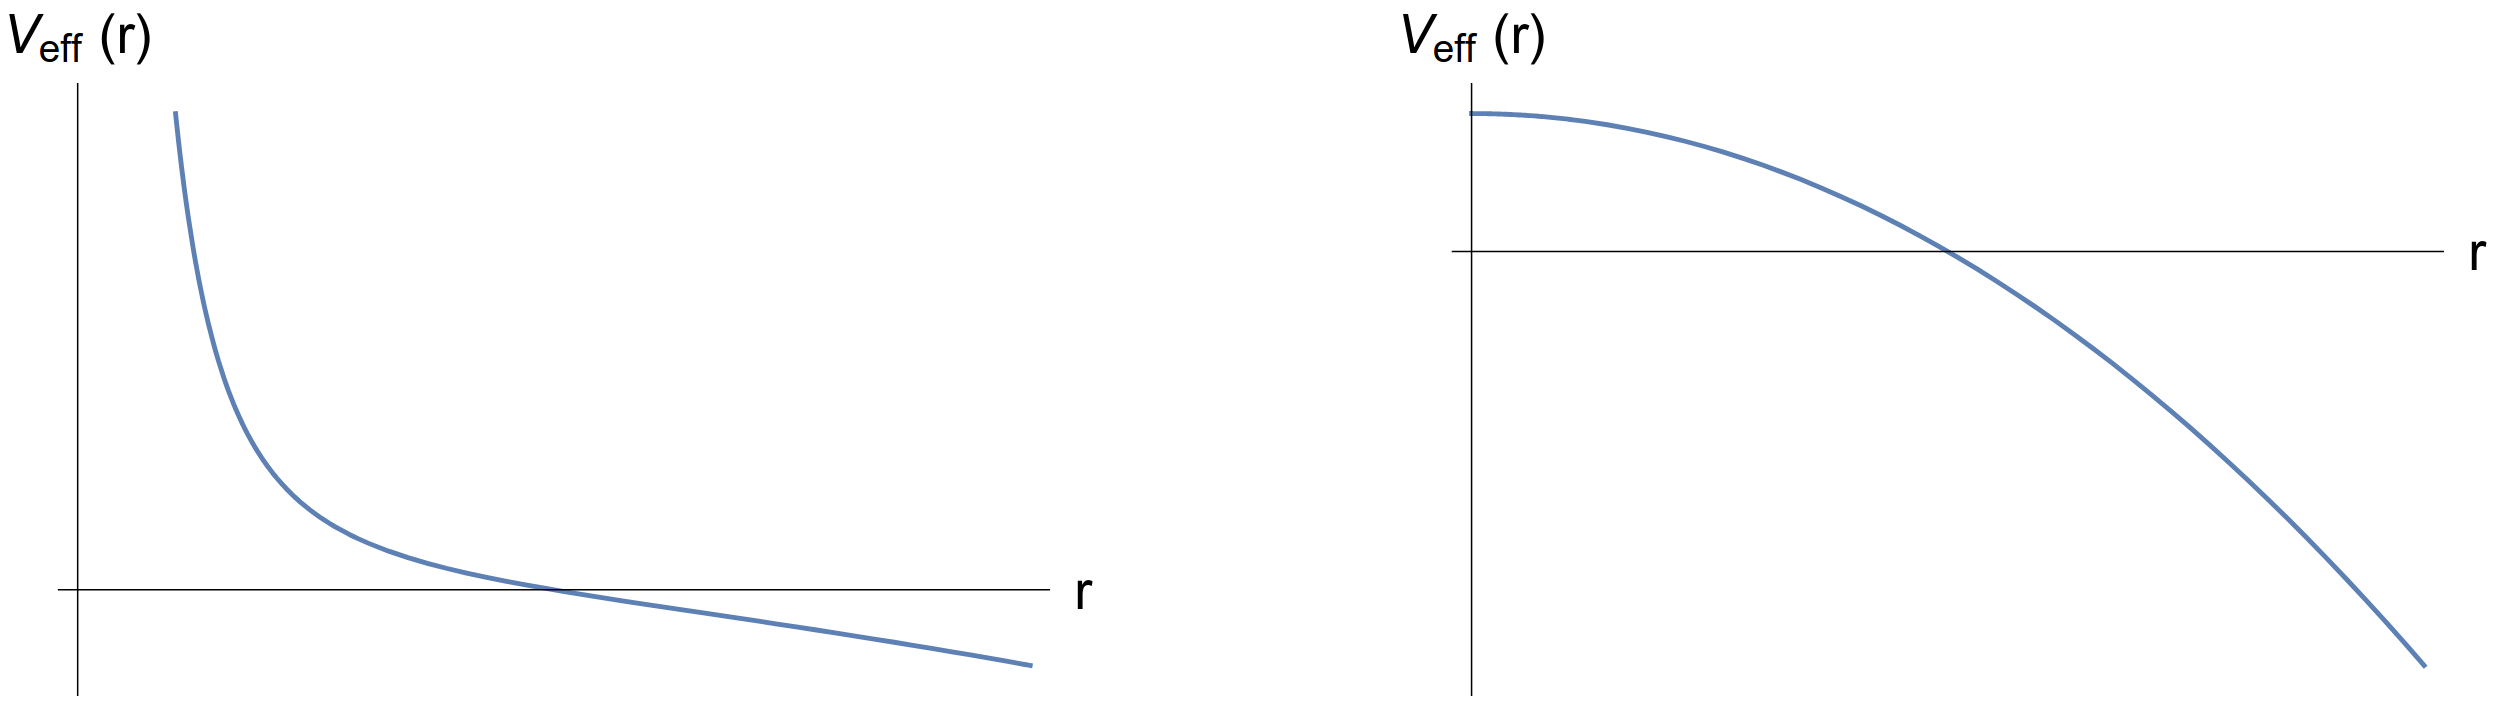
\includegraphics[width = 0.80 \textwidth]{geod-ds.png}
  \caption{Effective potential for de Sitter geodesics, with $ \ell \neq 0 $ and $ \ell = 0 $ respectively.}
  \label{geo-ds}
\end{figure}

For de Sitter space:
\begin{equation*}
  V_{\text{eff}}(r) = \left( 1 + \frac{\ell^2}{r^2} \right) \left( 1 - \frac{r^2}{R^2} \right)
\end{equation*}
This effective potential is plotted in Fig. \ref{geo-ds}: immediately, on sees that the potential pushes the particle to larger values of $ r $. Focusing on geodesics with $ \ell = 0 $, the potential is a harmonic repulsor: a particle stationary at $ r = 0 $ is an unstable geodesic, for if it has non-zero initial velocity it will follow the trajectory:
\begin{equation}
  r(\sigma) = R \sqrt{E^2 - 1} \sinh \frac{\sigma}{R}
  \label{eq:4.19}
\end{equation}
Note that the metric is singular at $ r = R $, a fact not manifest in the geodesic Eq. \ref{eq:4.19} which shows that any observer reaches $ r = R $ in finite proper time. Problems arise when studying the coordinate time $ t $, which has the interpretation of the time experienced by someone stationary at $ r = 0 $; from Eq. \ref{eq:4.16}:
\begin{equation*}
  \frac{dt}{d\sigma} = E \left( 1 - \frac{r^2}{R^2} \right)^{-1}
\end{equation*}
This shows that $ t(\sigma) \rightarrow \infty $ as $ r(\sigma) \rightarrow R $: in fact, if $ r(\sigma^*) = R $, then for $ \sigma = \sigma^* - \varepsilon $ one has $ \frac{dt}{d\sigma} = - \frac{\alpha}{\varepsilon} $, i.e. $ t(\varepsilon) = - \log (\varepsilon / R) $, so $ t(\varepsilon) \rightarrow \infty $ as $ \varepsilon \rightarrow 0 $. This means that a particle moving along the geodesic Eq. \ref{eq:4.19} will reach $ r = R $ in finite proper time, but a stationary observer at $ r = 0 $ will measure an infinite amount of time.\\
This strange behaviour is similar to what happens at the horizon of a black hole ($ r = 2GM $): however, the Schwarzschild metric has a singularity at $ r = 0 $, while de Sitter metric looks flat at $ r = 0 $. de Sitter space seems like an inverted black hole in which particles are pushed outwars to $ r = R $.

\subsubsection{de Sitter embeddings}

de Sitter space can be nicely embedded as a submanifold of $ \R^{1,4} $ with metric:
\begin{equation}
  ds^2 = - (dX^0)^2 + \sum_{i = 1}^{4} (dX^i)^2
  \label{eq:4.20}
\end{equation}
In particular, de Sitter metric Eq. \ref{eq:4.14} is a metric on the submanifold of $ \R^{1,4} $ defined by the timelike hyperboloid:
\begin{equation}
  -(X^0)^2 + \sum_{i = 1}^{4} (X^i)^2 = R^2
  \label{eq:4.21}
\end{equation}
A way of parametrizing this constraint is by imposing that $ r^2 = (X^1)^2 + (X^2)^2 + (X^3)^2 $, so that:
\begin{equation*}
  R^2 - r^2 = (X^4)^2 - (X^0)^2
\end{equation*}
The solutions are parametrized as:
\begin{equation*}
  X^0 = \sqrt{R^2 - r^2} \sinh \frac{t}{R}
  \qquad
  X^4 = \sqrt{R^2 - r^2} \cosh \frac{t}{R}
\end{equation*}
Computing the respective variations, along with $ \sum_{i = 1}^{3} (dX^i)^2 = dr^2 + r^2 d\Omega_2^2 $, where $ d\Omega_n^2 $ is the metric element on $ \mathbb{S}^n $, allows to show that the pull-back of the Minkowski metric Eq. \ref{eq:4.20} on the hyperboloid Eq. \ref{eq:4.21} so parametrized gives the de Sitter metric Eq. \ref{eq:4.14} in the static patch coordinates.\\
The coordinates $ \{X^i\}_{i = 0,\dots,4} $ so defined are not the most intuitive: they single out $ X^4 $ as special, when the constraint does no such thing, and they do not cover the whole hyperboloid, as they are limited to $ X^4 \ge 0 $. A better choice of parametrization is:
\begin{equation*}
  X^0 = R \sinh \frac{\tau}{T}
  \qquad \qquad
  X^i = y^i R \cosh \frac{\tau}{R}
  \,:\,
  \sum_{i = 1}^{4} (y^i)^2 = 1
\end{equation*}
Given this constraint, $ \{y^i\}_{i = 1,,2,3,4} $ parametrize $ \mathbb{S}^3 $. These coordinates retain more of the symmetry of de Sitter space and cover the whole space, thus are a better parametrization. The pull-back of Minkowski metric, however, gives a rather different metric on de Sitter space:
\begin{equation}
  ds^2 = - d\tau^2 + R^2 \cosh^2 \frac{\tau}{R}\, d\Omega_3^2
  \label{eq:4.22}
\end{equation}
These are known as \textit{global coordinates}, as they cover the whole space (except for singularities at the poles for any choice of coordinates on $ \mathbb{S}^3 $). Since this metric is related to that in Eq. \ref{eq:4.14} by a change of coordinates, it too must obey the Einstein equations. Global coordiantes also show that the singularity which happens at $ X^4 $, i.e. at $ r = R $, is nothing but a coordinate singularity.

\begin{figure}
  \centering
  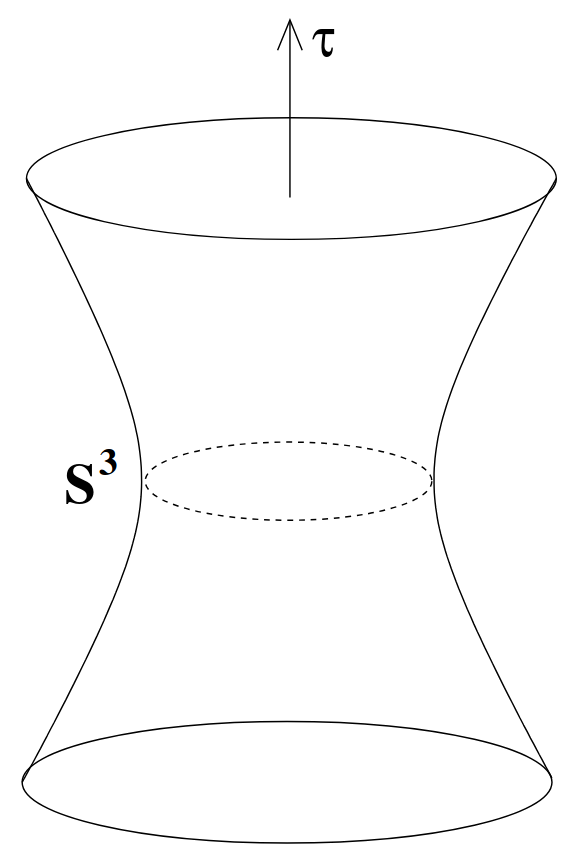
\includegraphics[width = 0.30 \textwidth]{ds-space.png}
  \caption{de Sitter space visualization with global coordinates.}
  \label{ds-space}
\end{figure}

These coordinates provide a clearer intuition for the physics of de Sitter space: it is a time-dependent solution of the field equations in which a spatial $ \mathbb{S}^3 $ first shrinks to a minimal radius $ R $ and then expands, as shown in Fig. \ref{ds-space}. The expansionary phase is a good approximation to our current universe on large scales.

\subsection{Anti-de Sitter space}

Consider $ \Lambda < 0 $. With the same ansatz as for de Sitter space, it's easy to find the metric for \textit{anti-de Sitter space} (AdS):
\begin{equation}
  ds^2 = - \left( 1 + \frac{r^2}{R^2} \right) dt^2 + \left( 1 + \frac{r^2}{R^2} \right)^{-1} dr^2 + r^2 d\Omega_2^2
  \qquad
  R^2 \equiv - \frac{3}{\Lambda}
  \label{eq:4.23}
\end{equation}
Equivalent coordinates are found setting $ r = R \sinh \rho $:
\begin{equation}
  ds^2 = - \cosh^2 \rho\, dt^2 + R^2 d\rho^2 + R^2 \sinh^2 \rho\, d\Omega_2^2
  \label{eq:4.24}
\end{equation}
In AdS there's no coordinate singularity in $ r $ and indeed now coordinates cover the whole space.

\subsubsection{Anti-de Sitter geodesics}

AdS has the same action as in Eq. \ref{eq:4.15}, thus the radial trajectory of a massive particle moving along a geodesic in the $ \vartheta = \frac{\pi}{2} $ plane is $ \dot{r}^2 + V_{\text{eff}}(r) = E^2 $, with:
\begin{equation}
  V_{\text{eff}}(r) = \left( 1 + \frac{\ell^2}{R^2} \right) \left( 1 + \frac{r^2}{R^2} \right)
  \label{eq:4.25}
\end{equation}

\begin{figure}
  \centering
  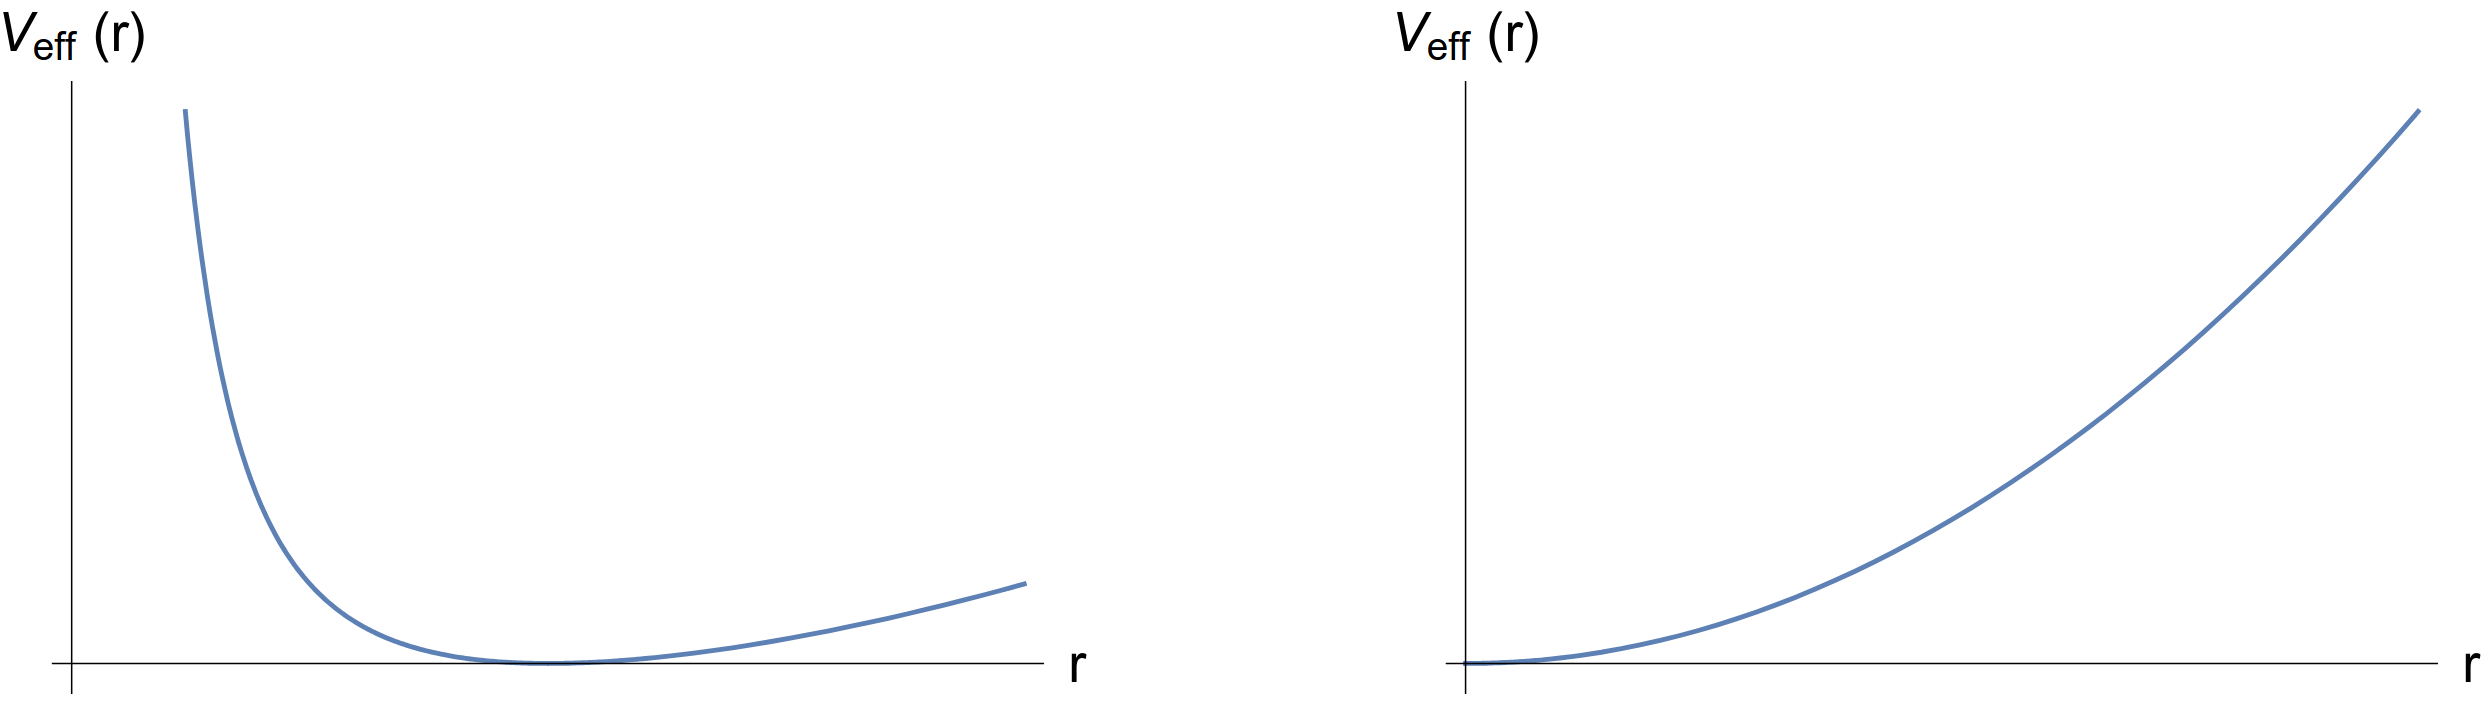
\includegraphics[width = 0.80 \textwidth]{geod-ads.png}
  \caption{Effective potential for anti-de Sitter geodesics, with $ \ell \neq 0 $ and $ \ell = 0 $ respectively.}
  \label{geo-ads}
\end{figure}

Plotting it in Fig. \ref{geo-ads}, the geodesics' behavior is clear: with no angular momentum, anti-de Sitter space acts like a harmonic oscillator, pulling the particle towards the origin and making it oscillate around $ r = 0 $. If the particle has non-zero angular momentum, then the potential has a minimum at $ r_*^2 = R \ell $, thus particles oscillate around $ r_* $: importantly, particles with finite energy cannot escape to $ r \rightarrow \infty $, but are constrained by the spacetime within some finite distance from the origin.\\
This picture of AdS as a harmonic trap which pulls particle to the origin clashes with the fact that AdS is a homogeneous space (roughly, all points are the same). To understand how these two facts are compatible, consider a stationary observer at $ r = 0 $: this is a geodesic and, from its perspective, other observers (with $ \ell = 0 $) will oscillate around $ r = 0 $ along geodesics. However, since these observers move along geodesics, in their reference frame they are stationary at $ r = 0 $, with all other observers oscillating. Thus, while in dS each observer views themselves at the center of the universe, with other observers moving away from them, in AdS each observer views themselves as the center of the universe, with other observer oscillating around them.\\
Its possible to study geodesics for a massless particle too. This time, the constraint to the action is:
\begin{equation*}
  - f(r)^2 \dot{t}^2 + f(r)^{-2} \dot{r}^2 + r^2 (\dot{\vartheta}^2 + \sin^2 \vartheta \dot{\varphi}^2) = 0
\end{equation*}
This means that the particle follows a null geodesic. Its equation of motion is:
\begin{equation*}
  \dot{r}^2 + V_{\text{null}}(r) = E^2
  \qquad
  V_{\text{null}}(r) = \frac{\ell^2}{r^2} \left( 1 + \frac{r^2}{R^2} \right)
\end{equation*}

\begin{figure}
  \centering
  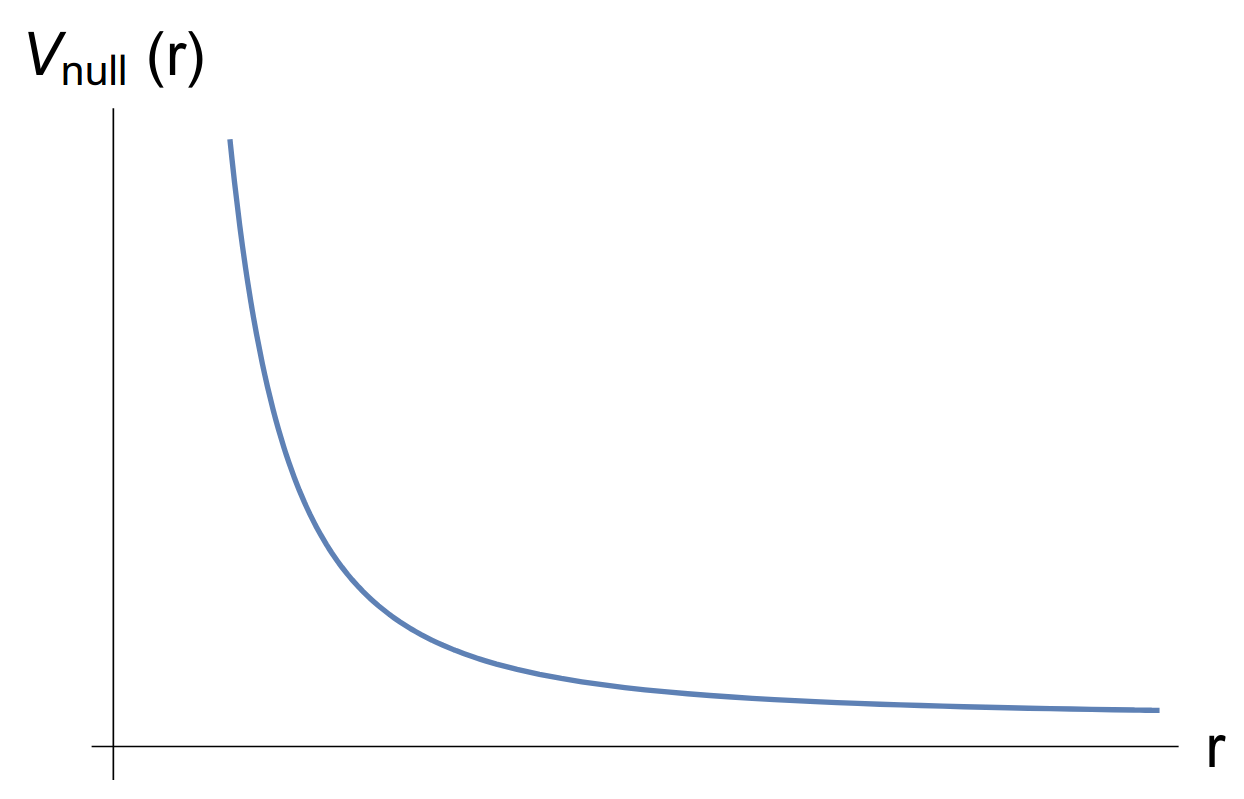
\includegraphics[width = 0.50 \textwidth]{ads-pot.png}
  \caption{Potential experienced by massless particles with $ \ell \neq 0 $ in AdS.}
  \label{ads-pot}
\end{figure}

Its plot in Fig. \ref{ads-pot} makes it clear that massless particle can escape to $ r \rightarrow \infty $, as the null potential is asymptotically constant, and it will only experience the usual gravitational redshift. AdS only confines massive particles.
To solve for the trajectory, it's easier to work with $ r = R \sinh \rho $ and $ \ell = 0 $, so that:
\begin{equation*}
  R \dot{\rho} = \pm \frac{E}{\cosh \rho}
  \quad \Rightarrow \quad
  R \sinh \rho(\sigma) = E (\sigma - \sigma_0)
\end{equation*}
One sees that $ \rho \rightarrow \infty $ only in infinite affine time (i.e. $ \sigma \rightarrow \infty $). However, in coordinate time, recalling Eq. \ref{eq:4.16}, $ E = \cosh^2 \rho\, \dot{t} $, so:
\begin{equation*}
  R \tan \frac{t}{R} = E (\sigma - \sigma_0)
\end{equation*}
Hence, as affine time $ \sigma \rightarrow \infty $, coordinate time $ t \rightarrow \frac{\pi}{2} R $. This means that light rays escape to infinity in a finite amount of coordinate time: to make sense of dynamics in AdS, one must specify some boundary conditions at infinity to dictate how massless particles and field behave.\\
AdS does not appear to be of any cosmological interest.

\subsubsection{Anti-de Sitter embeddings}

AdS too has a natural embedding in a 5d spacetime: it is a submanifold of $ \R^{2,3} $ with metric:
\begin{equation}
  ds^2 = - (dX^0)^2 - (dx^4)^2 + \sum_{i = 1}^{3} (dX^i)^2
  \label{eq:4.26}
\end{equation}
In particular, anti-de Sitter metric Eq. \ref{eq:4.23} is a metric on the hyperboloid:
\begin{equation}
  - (X^0)^2 - (X^4)^2 + \sum_{i = 1}^{3} (X^i)^2 = - R^2
  \label{eq:4.27}
\end{equation}
This constraint can be solved via the parametrization:
\begin{equation*}
  X^0 = R \cosh \rho \sin \frac{t}{R}
  \qquad
  X^4 = R \cosh \rho \cos \frac{t}{R}
  \qquad
  X^i = y^i R \sinh \rho
  \,:\,
  \sum_{i = 1}^{3} (y^i)^2 = 1
\end{equation*}
Given this constraint, $ \{y^i\}_{i = 1,2,3} $ parametrize $ \mathbb{S}^2 $. The pull-back of the metric Eq. \ref{eq:4.26} on the hyperboloid so parametrized gives anti-de Sitter metric Eq. \ref{eq:4.24}.\\
There's a small subtlety: the embedding hyperboloid has topology $ \mathbb{S}^1 \times \R^3 $, not $ \R^4 $: this corresponds to a compact time direction, as $ t \in [0, 2\pi R) $. However, AdS metric does not have such restriction, with $ t \in \R $: this is a universal covering of the hyperboloid.\\
Another useful parametrization of the hyperboloid is the following:
\begin{equation*}
  X^4 - X^3 = r
  \qquad
  X^4 + X^3 = \frac{R^2}{r} + \frac{r}{R^2} \eta_{ij} dx^i dx^j
  \qquad
  X^i = \frac{r}{R} x^i
  \,,\, i = 0,1,2
\end{equation*}
with $ r \in [0, \infty) $. With these coordinates, the metric takes the form:
\begin{equation*}
  ds^2 = R^2 \frac{dr^2}{r^2} + \frac{r^2}{R^2} \eta_{ij} dx^i dx^j
\end{equation*}
These coordinates don't cover the whole AdS, but only one-half of the hyperboloid, restricted to $ X^4 - X^3 > 0 $: this is known as the \textit{Poincaré patch} of AdS. Moreover, $ x^0 $ cannot be further extended beyond $ x^0 \in (-\infty, +\infty) $, thus in global coordinates the restriction $ t \in [0,2\pi R) $ remains. In this case, massive particles fall towards $ r = 0 $.\\
Finally, there are two more possible coordinate systems on the Poincaré patch, obtained by setting $ z = \frac{R^2}{r} $ and $ r = R e^\rho $:
\begin{equation*}
  ds^2 = \frac{R^2}{z^2} \left( dz^2 + \eta_{ij} dx^i dx^j \right)
  \qquad \qquad
  ds^2 = R^2 d\rho^2 + e^{2\rho} \eta_{ij} dx^i dx^j
\end{equation*}
In each case, massive particles fall towards $ z = \infty $ or $ \rho = -\infty $.

\section{Symmetries}

What makes Minkowski, dS and AdS special solutions to the Einstein equations are their symmetries.\\
The symmetries of Minkowski spacetime are familiar: translations and rotations of spacetime, with the latter splitting between proper rotations and Lorentz boosts. These symmetries are responsible for the existence of energy, momentum and angular momentum on a fixed Minkowski background.\\
It is important to characterize the symmetries of a general metric.

\subsection{Isometries}

Recall Def. \ref{def-flow} of flow on a manifold: by Eq. \ref{eq:2.10}, it is possible to identify a flow with a vector field $ K \in \xm $ such that it is tangent to the flow at each point of the manifold: $ K^\mu = \frac{dx^\mu}{dt} $, with $ x^\mu(t) \equiv x^\mu(\sigma_t) $.

\begin{definition}
  Given a flow associated to $ K \in \xm $, it is said to be an \textit{isometry} if:
  \begin{equation}
    \ld_K g = 0
    \quad \Leftrightarrow \quad
    \na_\mu K_\nu + \na_\nu K_\mu = 0
    \label{eq:4.28}
  \end{equation}
\end{definition}
Recall Eqq. \ref{eq:4.11}-\ref{eq:4.12} for the equivalence. This condition means that the metric doesn't change along flow lines: this is called \textit{Killing equation}, and a vector field which satisfied it is a \textit{Killing vector field}.
Prop. \ref{prop-lie-algebra} can be generalized to hold for the Lie derivative of arbitrary tensor fields, thus Killing vectors too form a Lie algebra: it is the Lie algebra of the isometry group of the manifold.

\begin{example}
  Given a metric $ g_{\mu \nu}(x) $, if it doesn't depend on $ x^1 \equiv y $, then $ X = \pa_y $ is a Killing vector field, for $ (\ld_{\pa_y} g)_{\mu \nu} = \pa_y g_{\mu \nu} = 0 $. This is the case of ignorable degrees of freedom, as in Eqq. \ref{eq:4.16}-\ref{eq:4.17}.
\end{example}

\subsubsection{Minkowski spacetime}

Consider Minkowski spacetime $ \R^{1,3} $ with $ g_{\mu \nu} = \eta_{\mu \nu} $. Killing equation is:
\begin{equation*}
  \pa_\mu K_\nu + \pa_\nu K_\mu = 0
\end{equation*}
There two forms of solution. The first one is:
\begin{equation*}
  K_\mu = c_\mu
\end{equation*}
for any constant vector $ c_\mu $. These generate translations. Alternatively:
\begin{equation*}
  K_\mu = \omega_{\mu \nu} x^\nu
  \,:\, \omega_{\mu \nu} = - \omega_{\nu \mu}
\end{equation*}
These generate rotations and Lorentz boosts. The emergence of the Lie algebra structure can be elucidated defining the Killing vectors:
\begin{equation*}
  P_\mu \defeq \pa_\mu
  \qquad
  M_{\mu \nu} \defeq \eta_{\mu \rho} x^\rho \pa_\nu - \eta_{\nu \rho} x^\rho \pa_\mu
\end{equation*}
These are 10 Killing vectors: 4 for translations and 6 for rotations and boosts.

\begin{proposition}
  Killing vectors of Minkowski spacetime obbey:
  \begin{equation*}
    [P_\mu, P_\nu] = 0
    \qquad
    [M_{\mu \nu}, P_\sigma] = - \eta_{\mu \sigma} P_\nu + \eta_{\sigma \nu} P_\mu
  \end{equation*}
  \begin{equation*}
    [M_{\mu \nu}, M_{\rho \sigma}] = \eta_{\mu \sigma} M_{\nu \rho} + \eta_{\nu \rho} M_{\mu \sigma} - \eta_{\mu \rho} M_{\nu \sigma} - \eta_{\nu \sigma} M_{\mu \rho}
  \end{equation*}
\end{proposition}
\begin{proof}
  By direct calculation.
\end{proof}

This is precisely the Lie algebra of the Poincaré group $ \R^4 \times \SOn{1,3} $, i.e. the isometry group of Minkowski spacetime.

\subsubsection{de Sitter and anti-de Sitter space}

The isometries of dS and AdS are best seen from their embeddings.
The constraint Eq. \ref{eq:4.21} which defined de Sitter space is invariant under the rotations of $ \R^{1,4} $, thus dS inherits the $ \SOn{1,4} $ isometry group. Similarly, the constraint Eq. \ref{eq:4.27} which defines anti-de Sitter space is invariant under rotations of $ \R^{2,3} $, so AdS inherits the $ \SOn{2,3} $ isometry group. Note that both these groups are 10-dimensional, as $ \R^4 \times \SOn{1,3} $.\\
It's simple to determine the 10 Killing spinors of 5d spacetime:
\begin{equation*}
  M_{AB} = \eta_{AC} X^C \pa_B - \eta_{BC} X^C \pa_A
\end{equation*}
where $ X^A, A = 0,1,2,3,4 $ are 5d coordinates and $ \eta_{AB} $ is the appropriate Minkowski metric, with signature $ (-,+,+,+,+) $ for dS and $ (-,-,+,+,+) $ for AdS. In either case, the Lie algebra is that of the appropriate Lorentz group:
\begin{equation*}
  [M_{AB}, M_{CD}] = \eta_{AD} M_{BC} + \eta_{BC} M_{AD} - \eta_{AC} M_{BD} - \eta_{BD} M_{AC}
\end{equation*}
The embedding hyperbolae are both invariant under these Killing vectors: flows generated by them map points on the hyperbolae to other points on the hyperbolae. Therefore, these Killing vectors are inherited by dS and AdS respectively.

\paragraph{Energy}

Energy is defined by timelike Killing vectors. In anti-de Sitter space there's no problem finding a timelike Killing vector, as the metric in global coordinates Eq. \ref{eq:4.24} is time-independent, so $ K = \pa_t $. However, this changes in de Sitter space.\\
Considering dS in the static patch with coordinates $ r^2 = (X^1)^2 + (X^2)^2 + (X^3)^2 $, $ X^0 = \sqrt{R^2 - r^2} \sinh \frac{t}{R} $ and $ X^4 = \sqrt{R^2 - r^2} \cosh \frac{t}{R} $, the metric Eq. \ref{eq:4.14} is time-independent, thus $ K = \pa_t $ is a Killing vector; pushing it forward to the 5d space:
\begin{equation*}
  \pa_t = \frac{\pa X^A}{\pa t} \pa_A = \frac{1}{R} ( X^4 \pa_0 + X^0 \pa_4 )
\end{equation*}
On the static patch, this Killing vector is timelike and the energy Eq. \ref{eq:4.16} follows from it. The problem is that the static patch is only one-half of the hyperboloid: when considering the whole AdS, one must account for the case $ X^0 = 0, X^4 < 0 $, in which the Killing vector points in the past direction, or $ X^0 \neq 0, X^4 = 0 $, in which it is spacelike. Therefore, the Killing vector can be both timelike (future-directed and past-directed) or spacelike when spanning the whole manifold: for this reason, it's not possible to define a global positive conserved energy on the total de Sitter space. The same conclusion follows by noting that the metric in global coordinates Eq. \ref{eq:4.22} is time-dependent.

\subsection{Conserved quantities}

It is possible to reframe Noether's theorem in the context of Killing vectors.

\begin{theorem}[Noether]
  Given a massive particle moving on a geodesic $ x^\mu(\tau) $ in a spacetime with metric $ g $ which admits a Killing vector field $ K $, then the \textit{Noether charge} is conserved along the geodesic:
  \begin{equation}
    Q \defeq K_\mu \frac{dx^\mu}{d\tau}
    \label{eq:4.29}
  \end{equation}
\end{theorem}
\begin{proof}
  First, show that $ Q $ is indeed conserved along the geodesic, recalling Eq. \ref{eq:4.28}:
  \begin{equation*}
    \frac{dQ}{d\tau} = \pa_\nu K_\mu \frac{dx^\nu}{d\tau} \frac{dx^\mu}{d\tau} + K_\mu \frac{d^2 x^\mu}{d\tau^2} = \pa_\nu K_\mu \frac{dx^\nu}{d\tau} - K_\mu \Gamma^\mu_{\rho \sigma} \frac{dx^\rho}{d\tau} \frac{dx^\sigma}{d\tau} = \na_\nu K_\mu \frac{dx^\nu}{d\tau} \frac{dx^\mu}{d\tau} = 0
  \end{equation*}
  To show that $ Q $ follows from Noether's theorem, consider the action of the massive particle and introduce an infinitesimal transformation $ \delta x^\mu = K^\mu (x) $:
  \begin{equation*}
    \begin{split}
      \delta \mathcal{S}
      &= \delta \int d\tau\, g_{\mu \nu}(x) \frac{dx^\mu}{d\tau} \frac{dx^\nu}{d\tau} = \int d\tau \left[ \pa_\rho g_{\mu \nu} \frac{dx^\mu}{d\tau} \frac{dx^\nu}{d\tau} \delta x^\rho + 2 g_{\mu \nu} \frac{dx^\mu}{d\tau} \frac{d \delta x^\nu}{d\tau} \right] \\
      &= \int d\tau \left[ \pa_\rho g_{\mu \nu} \frac{dx^\mu}{d\tau} \frac{dx^\nu}{d\tau} K^\rho + 2 \frac{dx^\mu}{d\tau} \left( \frac{dK_\mu}{d\tau} - K^\nu \frac{dg_{\mu \nu}}{d\tau} \right) \right] \\
      &= \int d\tau \left[ \pa_\rho g_{\mu \nu} K^\rho - 2 K^\rho \pa_\nu g_{\mu \rho} + 2 \pa_\nu K_\mu \right] \frac{dx^\mu}{d\tau} \frac{dx^\nu}{d\tau} = \int d\tau\, 2 \na_\nu K_\mu \frac{dx^\mu}{d\tau} \frac{dx^\nu}{d\tau}
    \end{split}
  \end{equation*}
  The transformation is a symmetry if $ \delta \mathcal{S} = 0 $, thus, by the symmetry of $ \frac{dx^\mu}{d\tau} \frac{dx^\nu}{d\tau} $, the resulting equation is $ \na_{(\nu} K_{\mu)} = 0 $, i.e. Killing equation.
\end{proof}

\begin{example}
  Energy and angular momentum defined on de Sitter geodesics by Eqq. \ref{eq:4.16}-\ref{eq:4.17} are Noether charges associated to Killing vectors $ \pa_t $ and $ \pa_\varphi $ respectively.
\end{example}

\subsection{Komar integrals}

\begin{definition}
  Given a Killing vector $ K = K^\mu \pa_\mu $, defined the 1-form $ K \equiv K_\mu dx^\mu $, the associated \textit{Komar form} is the 2-form defined as:
  \begin{equation}
    F \defeq dK
    \label{eq:4.30}
  \end{equation}
\end{definition}

\begin{proposition}
  Given a Killing vector $ K = K^\mu \pa_\mu $, the associated Komar form is:
  \begin{equation}
    F_{\mu \nu} = \na_\mu K_\nu - \na_\nu K_\mu
    \label{eq:4.31}
  \end{equation}
\end{proposition}
\begin{proof}
  $ F = \frac{1}{2} F_{\mu \nu} dx^\mu \wedge dx^\nu = dK = \na_\mu K_\nu dx^\mu \wedge dx^\nu $.
\end{proof}

\begin{theorem}
  If the vacuum Einstein equations $ R_{\mu \nu} = 0 $ hold, then a Komar form obeys the vacuum Maxwell equations:
  \begin{equation}
    d \star F = 0
    \quad \Leftrightarrow \quad
    \na^\mu F_{\mu \nu} = 0
    \label{eq:4.32}
  \end{equation}
\end{theorem}
\begin{proof}
  Recall Prop. \ref{prop-max-eq} for the equivalence. From Ricci identity Eq. \ref{eq:3.38}:
  \begin{equation*}
    (\na_\mu \nu_\nu - \na_\nu \na_\mu) K^\sigma = \tensor{R}{^\sigma_{\rho \mu \nu}} K^\rho
    \quad \Rightarrow \quad
    (\na_\mu \na_\nu - \na_\nu \na_\mu) K^\mu = R_{\rho \nu} K^\rho
  \end{equation*}
  From Killing equation $ \na_{(\mu} K_{\nu)} = 0 \,\Rightarrow\, \na_\mu K^\mu = 0 $, thus $ \na_\mu \na_\nu K^\mu = R_{\rho \nu} K^\rho $ and:
  \begin{equation*}
    \na^\mu F_{\mu \nu} = \na^\mu \na_\mu K_\nu - \na^\mu \na_\nu K_\mu = -2 \na^\mu \na_\nu K_\mu = -2 R_{\rho \nu} K^\rho
  \end{equation*}
  If $ R_{\rho \nu} = 0 $, then $ \na^\mu F_{\mu \nu} = 0 $.
\end{proof}

\begin{definition}
  Given a Komar form $ F $ associated to a Killing vector $ K $, the associated \textit{Komar charge} (or Komar integral) on a spatial submanifold $ \Sigma $ is defined as:
  \begin{equation}
    Q_{\text{Komar}} \defeq - \frac{1}{8\pi G} \int_\Sigma d \star F = - \frac{1}{8\pi G} \int_{\pa \Sigma} \star\, F = - \frac{1}{8\pi G} \int_{\pa \Sigma} \star\, dK
    \label{eq:4.33}
  \end{equation}
\end{definition}

\begin{proposition}
  If Eq. \ref{eq:4.32} holds, then $ Q_{\text{Komar}} $ is conserved.
\end{proposition}
\begin{proof}
  Recall Eq. \ref{eq:3.49}: the proof is identical.
\end{proof}

As for Noether integrals of a particle, Komar integrals of spacetime are interpreted based on the defining Killing vector. For example, if $ K^\mu $ is everywhere timelike, i.e. $ g_{\mu \nu} K^\mu K^\nu < 0 $, then its Komar integral can be identified with the energy (or the mass) of spacetime; if the Killing vector is related to rotations, instead, the conserved charge is the angular momentum of spacetime.

\section{Asymptotics of spacetime}

The three special solution (Minkowski, dS, AdS) not only have different spacetime curvature and symmetries, but, more fundamentally, they have different behavior at infinity. Their importance lie in the fact that, however complicated the metric might be, if fields are suitably localized, then they will asymptote to one of these three symmetric spaces.

\subsection{Conformal transformations}

\begin{definition}
  Given a metric manifold $ (\mathcal{M},g) $ and a non-vanishing $ \Omega \in \cm $, a \textit{conformal transformation} is defined as:
  \begin{equation}
    \tilde{g}_{\mu \nu}(x) = \Omega^2(x) g_{\mu \nu}(x)
    \label{eq:4.34}
  \end{equation}
\end{definition}

Typically, $ g $ and $ \tilde{g} $ describe different spacetime with considerably warped distances. However, conformal transformations preserve angles: in Lorentzian spacetime, the two metrics have the same causal structure, i.e. null/timelike/spacelike vector fields in one metric remain null/timelike/spacelike in the other too.

\begin{proposition}
  Only conformal transformations of the metric preserve its causal structure.
\end{proposition}

Although timelike particle trajectories necessarily remain timelike under a conformal transformation, the same needs not be true for geodesics, as distances get warped.

\begin{proposition}
  Null geodesics are mapped to null geodesics under a conformal transformation.
\end{proposition}
\begin{proof}
  First compute the Christoffel symbols in the new metric:
  \begin{equation*}
    \begin{split}
      \Gamma^\mu_{\rho \sigma}[\tilde{g}]
      &= \frac{1}{2} \tilde{g}^{\mu \nu} (\pa_\rho \tilde{g}_{\nu \sigma} + \pa_\sigma \tilde{g}_{\rho \nu} - \pa_\nu \tilde{g}_{\rho \sigma}) \\
      &= \frac{1}{2} \Omega^{-2} g^{\mu \nu} (\pa_\rho (\Omega^2 g_{\nu \sigma}) + \pa_\sigma (\Omega^2 g_{\rho \nu}) - \pa_\nu (\Omega^2 g_{\rho \sigma})) \\
      &= \Gamma^\mu_{\rho \sigma}[g] + \Omega^{-1} (\delta^\mu_\sigma \na_\rho \Omega + \delta^\mu_\rho \na_\sigma \Omega - g_{\rho \sigma} \na^\mu \Omega)
    \end{split}
  \end{equation*}
  In the last line, recall that $ \na = \pa $ on scalar functions. Suppose an affinely parametrized geodesic in the metric $ g $:
  \begin{equation*}
    \frac{d^2 x^\mu}{d\tau^2} + \Gamma^\mu_{\rho \sigma}[g] \frac{dx^\rho}{d\tau} \frac{dx^\sigma}{d\tau} = 0
    \quad \Rightarrow \quad
    \frac{dx^2 x^\mu}{d\tau^2} + \Gamma^\mu_{\rho \sigma}[\tilde{g}] \frac{dx^\rho}{d\tau} \frac{dx^\sigma}{d\tau} = \Omega^{-1} (\delta^\mu_\sigma \na_\rho \Omega + \delta^\mu_\rho \na_\sigma \Omega - g_{\rho \sigma} \na^\nu \Omega) \frac{dx^\rho}{d\tau} \frac{dx^\sigma}{d\tau}
  \end{equation*}
  For a null geodesic $ g_{\rho \sigma} \frac{dx^\rho}{d\tau} \frac{dx^\sigma}{d\tau} = 0 $, thus:
  \begin{equation*}
    \frac{dx^2 x^\mu}{d\tau^2} + \Gamma^\mu_{\rho \sigma}[\tilde{g}] \frac{dx^\rho}{d\tau} \frac{dx^\sigma}{d\tau} = 2 \frac{dx^\mu}{d\tau} \frac{1}{\Omega} \frac{d\Omega}{d\tau}
  \end{equation*}
  This is the equation of non-affinely parametrized geodesic (like Eq. \ref{eq:1.16}), hence the thesis.
\end{proof}

Usual curvature tensors are not invariant under conformal transformations. A curvature tensor that is indeed invariant is the \textit{Weyl tensor}:
\begin{equation}
  C_{\mu \nu \rho \sigma} \defeq R_{\mu \nu \rho \sigma} - \frac{2}{n - 2} \left( g_{\mu [\rho} R_{\sigma] \nu} - g_{\nu [\rho} R_{\sigma] \mu} \right) + \frac{2}{(n-1)(n-2)} R g_{\mu [\rho} g_{\sigma] \nu}
  \label{eq:4.35}
\end{equation}
where $ n \equiv \dim_{\R}\mathcal{M} $. The Weyl tensor has all the symmetries of the Riemann tensor, with the additional property that it vanishes when contracting any pair of indices with the metric: it can be viewed as the trace-free part of the Riemann tensor.

\subsection{Penrose diagrams}

To study the asymptotic behavior of spacetime, one needs to perform a conformal transformation that maps infinity to a finite distance: the resulting causal structure can then be drawn on a finite area and the resulting picture is called a \textit{Penrose diagram}.

\subsubsection{Minkowski spacetime}

It is simplest to study $ \R^{1,1} $, where the Minkowski metric is $ ds^2 = -dt^2 + dx^2 $. First, introduce \textit{lightcone coordinates}:
\begin{equation*}
  u = t - x
  \qquad
  v = t + x
  \quad \Rightarrow \quad
  ds^2 = - du\, dv
\end{equation*}
These coordinates range in $ u,v \in \R $. To work with finite quantities, define:
\begin{equation*}
  u = \tan \tilde{u}
  \qquad
  v = \tan \tilde{v}
  \quad \Rightarrow \quad
  ds^2 = - \frac{1}{\cos^2 \tilde{u}\, \cos^2 \tilde{v}} d\tilde{u}\, d\tilde{v}
\end{equation*}
where now $ \tilde{u},\tilde{v} \in \left( -\frac{\pi}{2}, +\frac{\pi}{2} \right) $. Note that the metric diverges when approaching the boundary of Minkowski spacetime. However, a conformal transformation is possible with $ \Omega(\tilde{u},\tilde{v}) \equiv \cos \tilde{u}\, \cos \tilde{v} $:
\begin{equation*}
  d\tilde{s}^2 = \left( \cos^2 \tilde{u}\, \cos^2 \tilde{v} \right) ds^2 = - d\tilde{u}\, d\tilde{v}
\end{equation*}
It is now possible to add $ \tilde{u} = \pm \frac{\pi}{2} $ and $ \tilde{v} = \pm \frac{\pi}{2} $: this operation is called \textit{conformal compactification}.

\begin{figure}
  \centering
  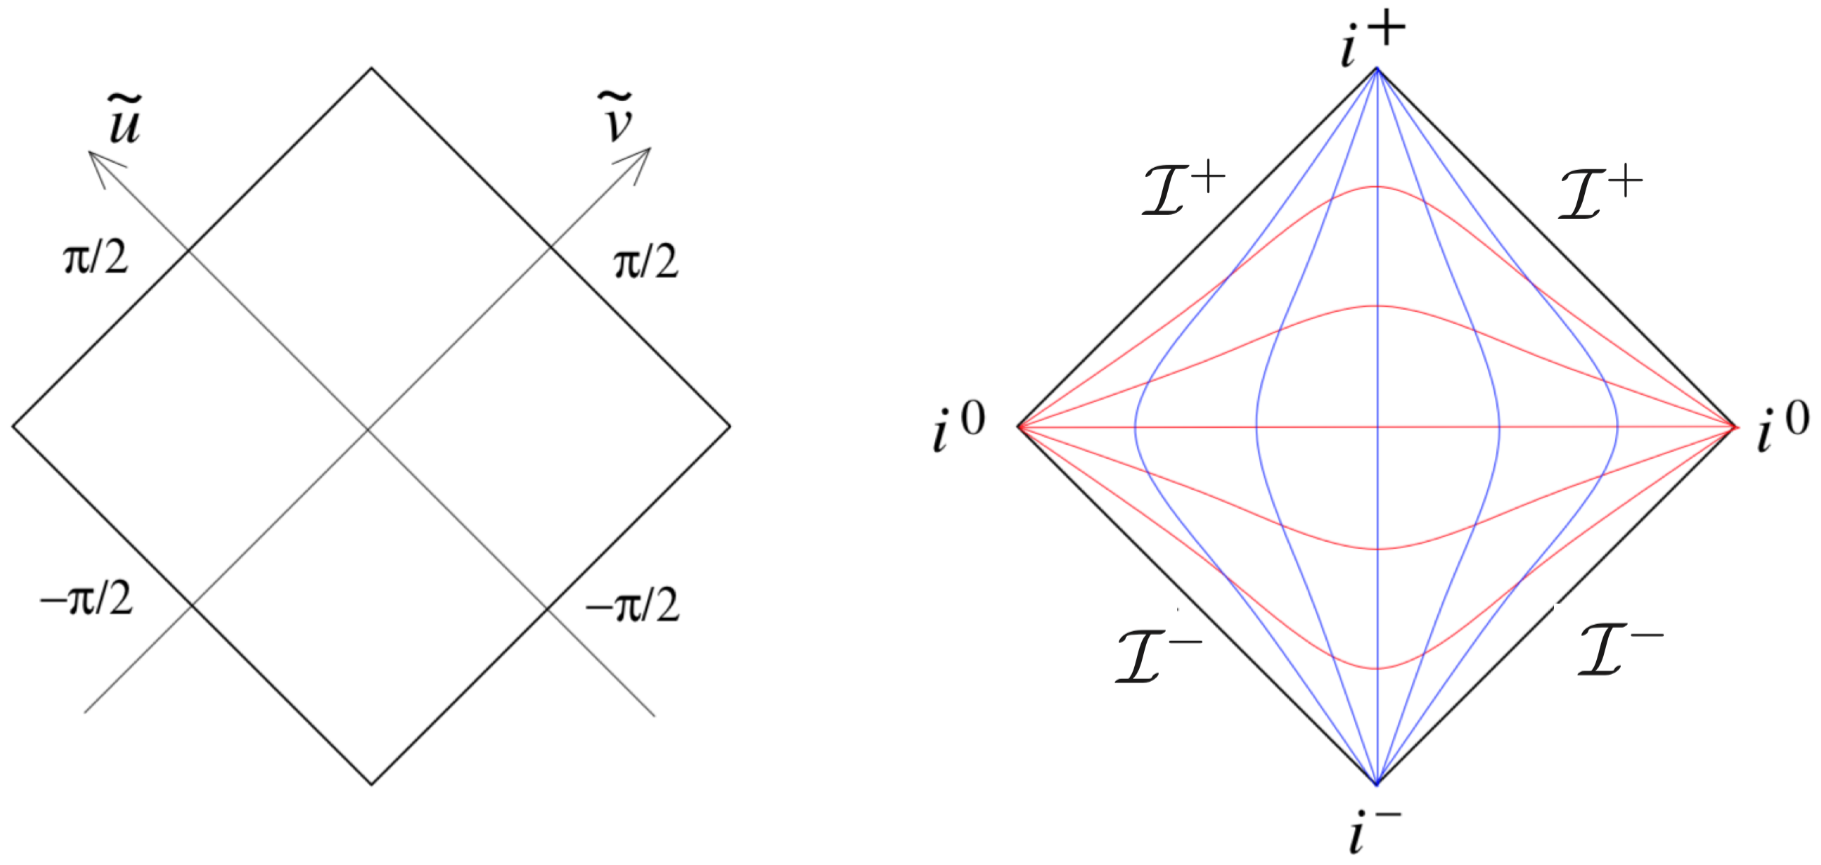
\includegraphics[width = 0.70 \textwidth]{ms-causal.png}
  \caption{Penrose diagram for $ d = 1 + 1 $ Minkowski spacetime.}
  \label{ms-causal}
\end{figure}

Penrose diagrams, as other relativistic diagrams, present light-rays travelling at 45°, time in the vertical direction and space in the horizontal one. Fig. \ref{ms-causal} shows the Penrose diagram for Minkowski spacetime $ \R^{1,1} $ with $ \tilde{u},\tilde{v} $ coordinates, both with coordinate axis and geodesics. Moreover, the various infinities of Minkowski space are shown:
\begin{itemize}
  \item timelike geodesics (blue) start at $ i^- (\tilde{u},\tilde{v}) = \left( -\frac{\pi}{2}, -\frac{\pi}{2} \right) $ and end at $ i^+ (\tilde{u},\tilde{v}) = \left( +\frac{\pi}{2}, +\frac{\pi}{2} \right) $, called respectively \textit{past} and \textit{future timelike infinity};
  \item spacelike geodesics (red) start and end at $ i^0 (\tilde{u},\tilde{v}) = \left( \mp \frac{\pi}{2}, \pm \frac{\pi}{2} \right) $, both called \textit{spacelike infinity};
  \item all null curves (not shown) start at the boundary $ \mathcal{I}^- \equiv \{\tilde{u} = - \frac{\pi}{2}\} \cup \{\tilde{v} = - \frac{\pi}{2}\} $ and end at the boundary $ \mathcal{I}^+ \equiv \{\tilde{u} = +\frac{\pi}{2}\} \cup \{\tilde{v} = +\frac{\pi}{2}\} $, called respectively \textit{past} and \textit{future null infinity}.
\end{itemize}
It's clear that in Minkowski spacetime there are more ways reach infinity along a null direction than in a timelike or spacelike direction.

\begin{figure}
  \centering
  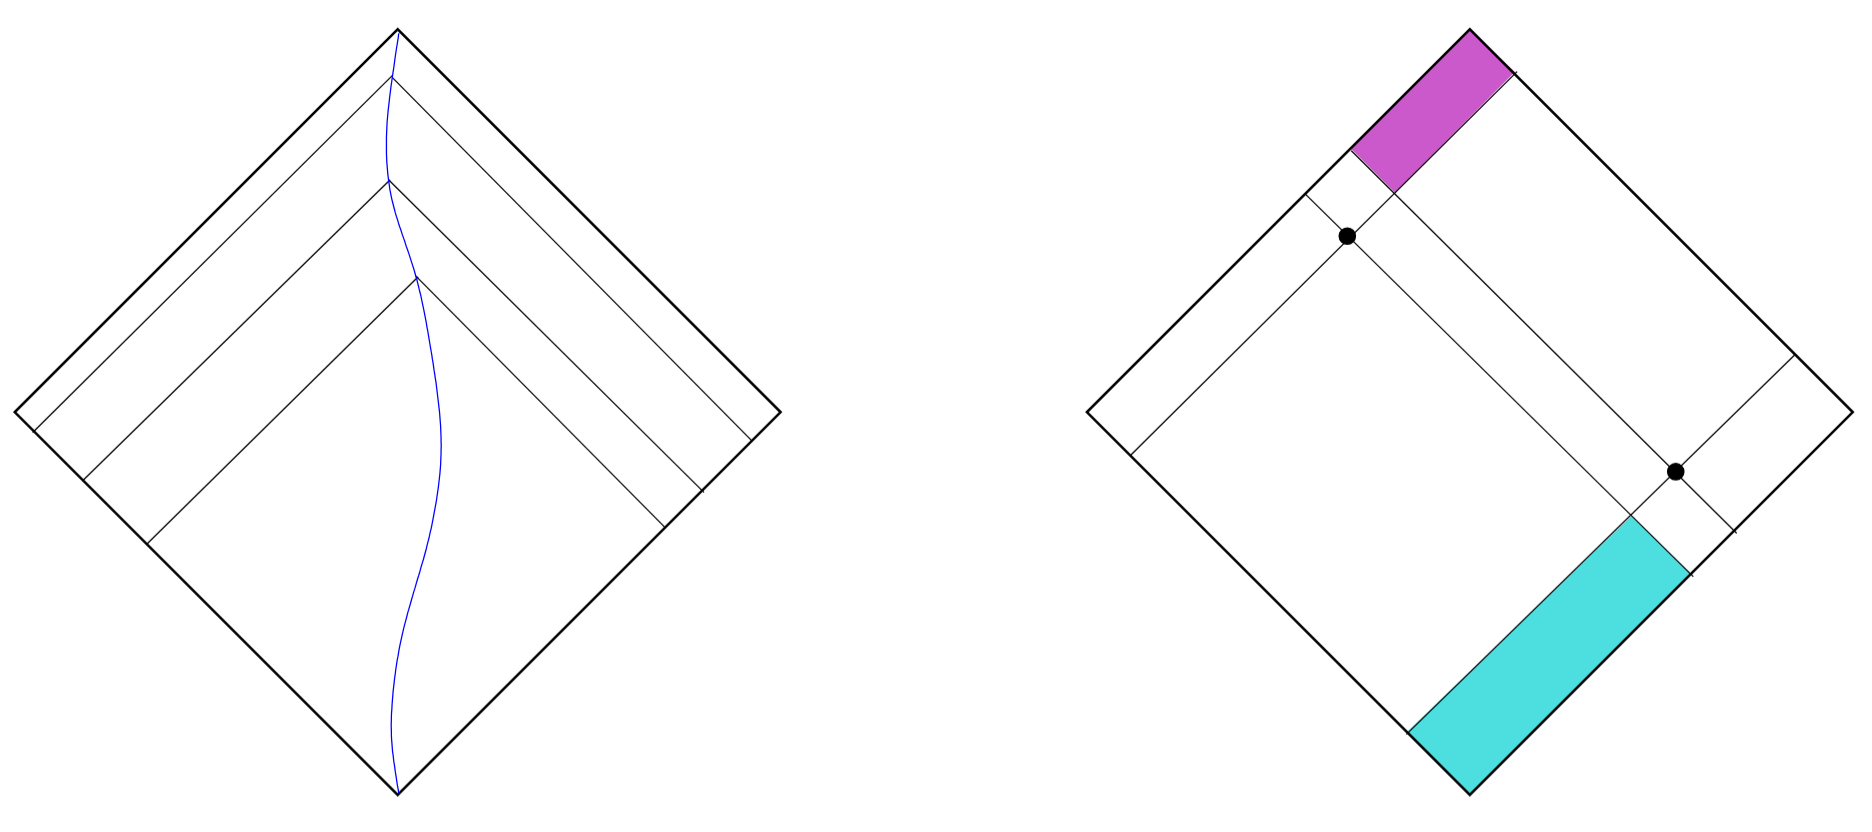
\includegraphics[width = 0.70 \textwidth]{ms-light.png}
  \caption{Lightcones in $ d = 1 + 1 $ Minkowski spacetime.}
  \label{ms-light}
\end{figure}

Penrose diagrams allow to immediately visualize the causal structure of spacetime. As shown in Fig. \ref{ms-light}, given a particle moving along a timelike curve, as it approaches $ i^+ $ its past lightcone encompasses progressively more of spacetime: thus, an observer in Minkowski spacetime can in principle see everything, as long as they wait long enough. Relatedly, given any two points in Minkowski spacetime, they are causally connected both in the past and in the future, as both cones intersect (see Fig. \ref{ms-light}): thus, there was always an event in the past that could have influenced both, and there will always be an event in the future that can be influenced by both.

\paragraph{4d Minkowski spacetime}

The analysis can be repeated for $ \R^{1,3} $ with $ ds^2 = -dt^2 + dr^2 + r^2 d\Omega_2^2 $. Lightcone coordinates are again:
\begin{equation*}
  u = t - r
  \qquad
  v = t + r
  \quad \Rightarrow \quad
  ds^2 = - du\, dv + \frac{1}{4} \left( u - v^2 \right) d\Omega_2^2
\end{equation*}
Finite range coordinates are again:
\begin{equation*}
   u = \tan \tilde{u}
  \qquad
  v = \tan \tilde{v}
  \quad \Rightarrow \quad
  ds^2 = \frac{1}{4\cos^2 \tilde{u}\, \cos^2 \tilde{v}} \left( -4 d\tilde{u}\, d\tilde{v} + \sin^2 (\tilde{u} - \tilde{v}) d\Omega_2^2 \right)
\end{equation*}
Finally, the conformal transformation with $ \Omega(\tilde{u},\tilde{v}) = 2 \cos \tilde{u}\, \cos \tilde{v} $ leads to:
\begin{equation*}
  d\tilde{s}^2 = - 4 d\tilde{u}\, d\tilde{v} + \sin^2 (\tilde{u} - \tilde{v}) d\Omega_2^2
\end{equation*}
In 4d Minkowski spacetime there's an additional constraint: $ r \ge 0 $, so $ v \ge v $. Conformal compactification leads to:
\begin{equation*}
  - \frac{\pi}{2} \le \tilde{u} \le \tilde{v} \le + \frac{\pi}{2}
\end{equation*}

\begin{figure}
  \centering
  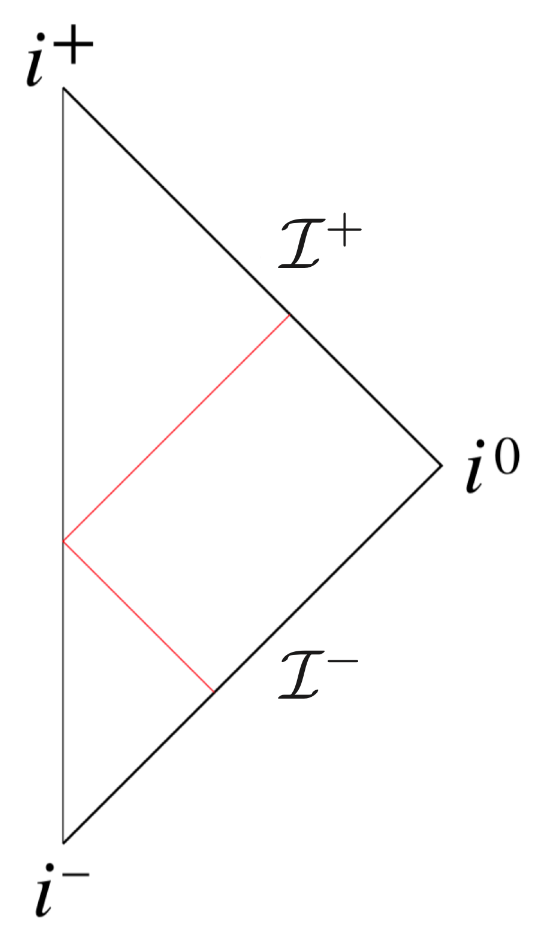
\includegraphics[width = 0.30 \textwidth]{ms-4d.png}
  \caption{Penrose diagram for $ d = 1 + 3 $ Minkowski spacetime.}
  \label{ms-4d}
\end{figure}

The corresponding Penrose diagram is drawn in Fig. \ref{ms-4d}: the spatial $ \mathbb{S}^2 $ is not shows for simplicity, but every point on the diagram corresponds to an $ \mathbb{S}^2 $ of radius $ \abs{\sin (\tilde{u} - \tilde{v})} $. The line $ \tilde{u} = \tilde{v} $ is not a boundary of Minkowski spacetime, but it's simply the origin $ r = 0 $ (at which $ \mathcal{S}^2 $ shrinks to a point): to illustrate this, a null geodesic is drawn.\\
In general, Penrose diagrams are only useful for spacetimes which contain an obvious $ \mathcal{S}^2 $, i.e. those with $ \SOn{3} $ isometry: however, these are the simplest and most important in physics.

\subsubsection{de Sitter space}

\begin{figure}
  \centering
  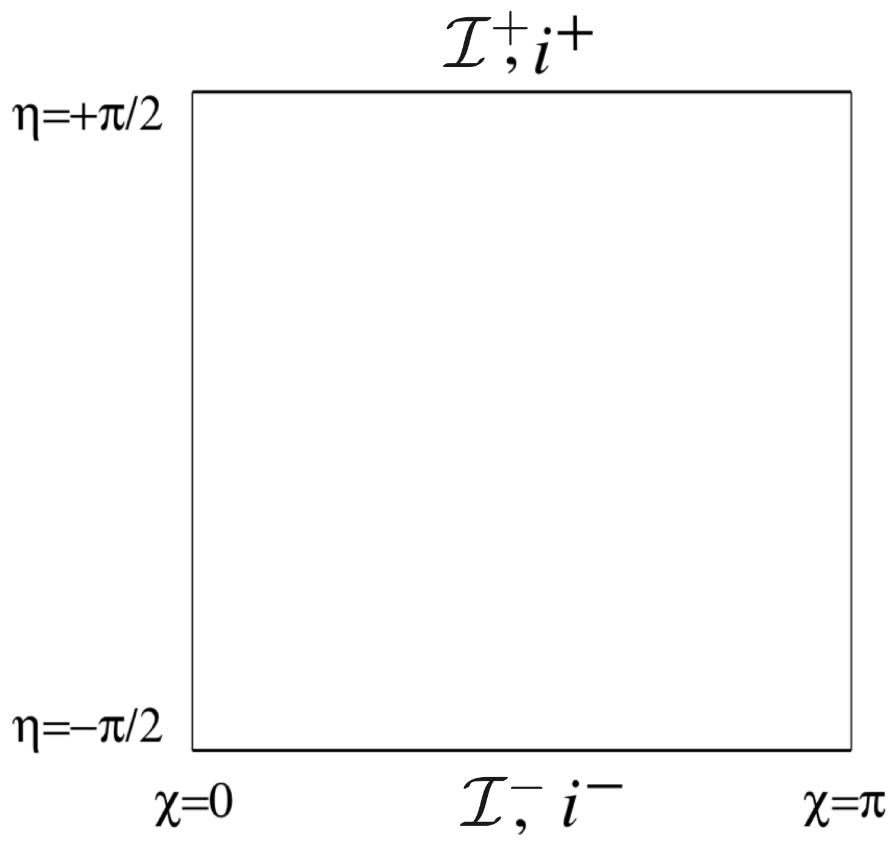
\includegraphics[width = 0.50 \textwidth]{ds-penr.png}
  \caption{Penrose diagram for de Sitter space.}
  \label{ds-penr}
\end{figure}

Recall global coordinates on dS: from Eq. \ref{eq:4.22}, $ ds^2 = -d\tau^2 + R^2 \cosh^2 \frac{\tau}{R} d\Omega_3^2 $. To draw the Penrose diagram, define \textit{conformal time} as:
\begin{equation*}
  \frac{d\eta}{d\tau} = \frac{1}{R \cosh (\tau / R)}
  \quad \Rightarrow \quad
  \cos \eta = \frac{1}{\cosh (\tau / R)}
\end{equation*}
Given that $ \tau \in \R $, then $ \eta \in \left( -\frac{\pi}{2}, +\frac{\pi}{2} \right) $. In conformal time, de Sitter space has the metric:
\begin{equation*}
  ds^2 = \frac{R^2}{\cos^2 \eta} \left( -d\eta^2 + d\Omega_3^2 \right)
\end{equation*}
Writing $ d\Omega_3^2 = d\chi^2 + \sin^2 \chi\, d\Omega_2^2 $, with $ \chi \in [0,\pi] $, de Sitter metric is conformally equivalent to:
\begin{equation*}
  d\tilde{s}^2 = -d\eta^2 + d\chi^2 + \sin^2 \chi\, d\Omega_2^2
\end{equation*}
After conformal compactification, $ \eta \in \left[ - \frac{\pi}{2}, + \frac{\pi}{2} \right] $ and $ \chi \in \left[ 0,\pi \right] $. The Penrose diagram is drawn in Fig. \ref{ds-penr}: the two vertical lines are not boundaries of dS, but simply the north and south poles of $ \mathbb{S}^3 $. The boundaries of the spacetime are the top and bottom lines, labelled both $ i^{\pm} $ and $ \mathcal{I}^{\pm} $ as they are where both timelike and null geodesics originate and terminate.

\begin{figure}
  \centering
  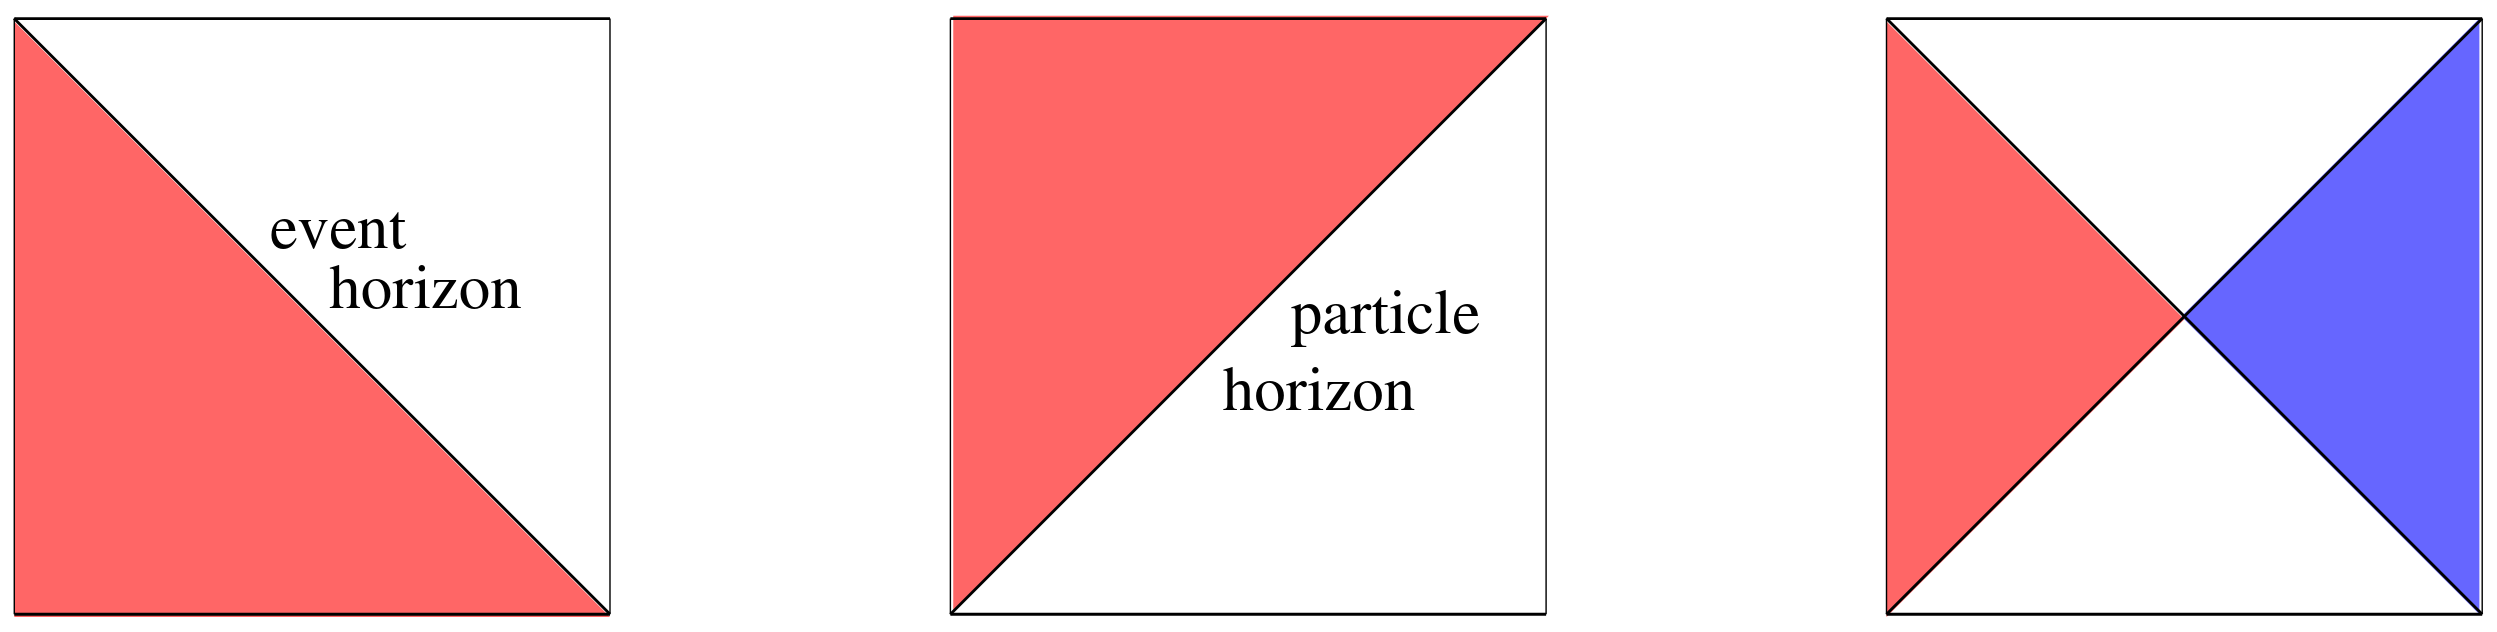
\includegraphics[width = 0.80 \textwidth]{ds-diam.png}
  \caption{Event and particle horizons for an observer at the north pole in dS, and the causal diamonds for an observer at the north and south pole.}
  \label{ds-diam}
\end{figure}

\begin{proposition}
  de Sitter spacetime has a \textit{spacelike} $ \mathbb{S}^3 $ boundary with timelike normal vector.
\end{proposition}

The causal structure of dS is very different from that of Minkowski spacetime: it is no longer true that any observer can see everything by waiting long enough. For example, as shown in Fig. \ref{ds-diam}, an observer at the north pole will eventually see only exactly half the spacetime: the boundary of this half-space is the observer's \textit{event horizon}, in the sense that signals from beyond the horizon cannot reach them. It is also clear that this event horizon is observer-dependent: in this context, these are referred to as \textit{cosmological horizons}.\\
Furthermore, an observer at the north pole will only be able to communicate with another half of the spacetime, as shown in Fig. \ref{ds-diam}: the boundary of this region of influence is known as the \textit{particle horizon} and it represents the furthest distance light can travel since the beginning of time. Its intersection with the event horizon determines the (nothern) \textit{causal diamond}: usually, nothern and southern causal diamonds are causally disconnected.\\
Penrose diagrams can also be used to explain the divergence at $ r = R $ of the metric Eq. \ref{eq:4.14} on the static patch of dS. Recalling the embedding of the static patch in $ \R^{1,4} $, parametrized as $ X^0 = \sqrt{R^2 - r^2} \sinh \frac{t}{R} $ and $ X^4 = \sqrt{R^2 - r^2} \cosh \frac{t}{R} $. Naively the surface $ r = R $ corresponds to $ X^0 = X^4 = 0 $, but writing $ r = R ( 1 - \varepsilon^2 / 2) $ yields that $ X^0 \sim R \varepsilon \sinh \frac{t}{R} $ and $ X^4 \sim R \varepsilon \cosh \frac{t}{R} $, so $ \varepsilon \rightarrow 0 $ can be obtained keeping $ X^0, X^4 \neq 0 $ and finite, provided that $ t \rightarrow \pm \infty $: to do this, $ \varepsilon \exp (\pm t / R) $ must be kept finite, thus the surface $ r = R $ is identified with the lines $ X^0 = \pm X^4 $. Translation to polar coordinates is done by $ X^0 = R \sinh \frac{\tau}{R} $ and $ X^4 = R \cosh \frac{\tau}{R} \cos \chi $, with $ \chi $ the polar angle on $ \mathbb{S}^3 $; after mapping to conformal time, one finds that:
\begin{equation*}
  X^0 = \pm X^4
  \quad \Leftrightarrow \quad
  \sin \eta = \pm \cos \chi
  \quad \Leftrightarrow \quad
  \chi = \pm \left( \eta - \frac{\pi}{2} \right)
\end{equation*}
These are precisely the lines determining the polar causal diamonds. It can also be checked that $ r = R $ on the static patch corresponds to the north pole $ \chi = 0 $ in global coordinates and that $ t = \tau $ along this line. Therefore, the static patch of dS provides coordinates that cover only the nothern causal diamond of dS spacetime, with the coordinate singularity at $ r = R $ corresponding to the past and future observer-dependent horizons.

\begin{figure}
  \centering
  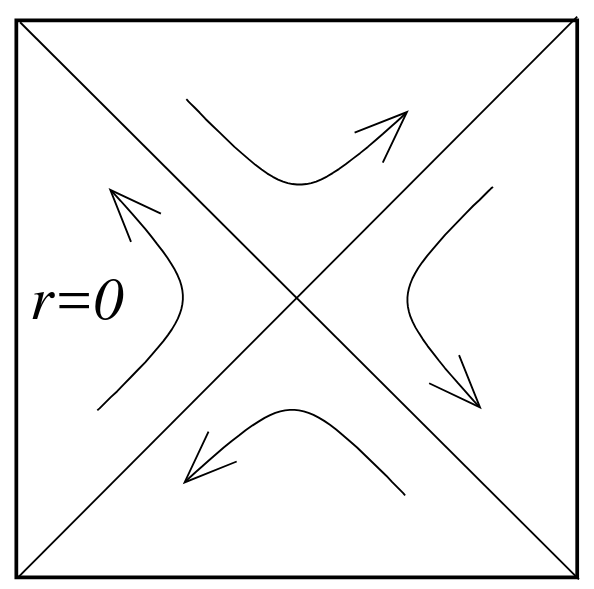
\includegraphics[width = 0.30 \textwidth]{ds-kill.png}
  \caption{$ K = \pa_t $ Killing vector field in de Sitter spacetime.}
  \label{ds-kill}
\end{figure}

Finally, Penrose diagrams help to understand the nature of the $ K = \pa_t $ Killing vector field exhibited by the static patch metric. As shown in Fig. \ref{ds-kill}, there's no global timelike Killing vector field in dS spacetime: extending the Killing vector beyond the static patch, i.e. the nothern causal diamond, it is timelike but past-oriented on the souther causal diamond and spacelike on the upper and lower quadrants.

\subsubsection{Anti-de Sitter space}

The global coordinates on AdS are, from Eq. \ref{eq:4.24}, $ ds^2 = - \cosh^2 \rho \, dt^2 + R^2 d\rho^2 + R^2 \sinh^2 \rho \, d\Omega_2^2 $, with $ \rho \in [0,\infty) $. Introduce a conformal radial coordinate:
\begin{equation*}
  \frac{d\psi}{d\rho} = \frac{1}{\cosh \rho}
  \quad \Rightarrow \quad
  \cos \psi = \frac{1}{\cosh \rho}
\end{equation*}
with $ \psi \in [0, \frac{\pi}{2}) $. With a dimensionless coordiante time $ \tilde{t} = \frac{t}{R} $, the metric becomes:
\begin{equation*}
  ds^2 = \frac{R^2}{\cos^2 \psi} \left( -d\tilde{t}^2 + d\psi^2 + \sin^2 \psi \, d\Omega_2^2 \right) = \frac{R^2}{\cos^2 \psi} \left( -d\tilde{t}^2 + d\Omega_3^2 \right)
\end{equation*}
AdS metric is conformally equivalent to:
\begin{equation*}
  d\tilde{s}^2 = -d\tilde{t}^2 + d\psi^2 + \sin^2 \psi \, d\Omega_2^2
\end{equation*}
After conformal compactification, $ \tilde{t} \in \R $ and $ \psi \in \left[ 0, \frac{\pi}{2} \right] $ and the resulting Penrose diagram is the infinite strip in Fig. \ref{ads-penr}. The edge at $ \psi = 0 $ is not a boundary, but the spatial origin where $ \mathcal{S}^2 $ shrinks to a point; in contrast, $ \psi = \frac{\pi}{2} $ is a boundary of the spacetime, labelled $ \mathcal{I} $, which should be viewed as a combination of $ \mathcal{I}^- $, $ \mathcal{I}^+ $ and $ i^0 $, since null and spacelike geodesics begin and end there.

\begin{figure}
  \centering
  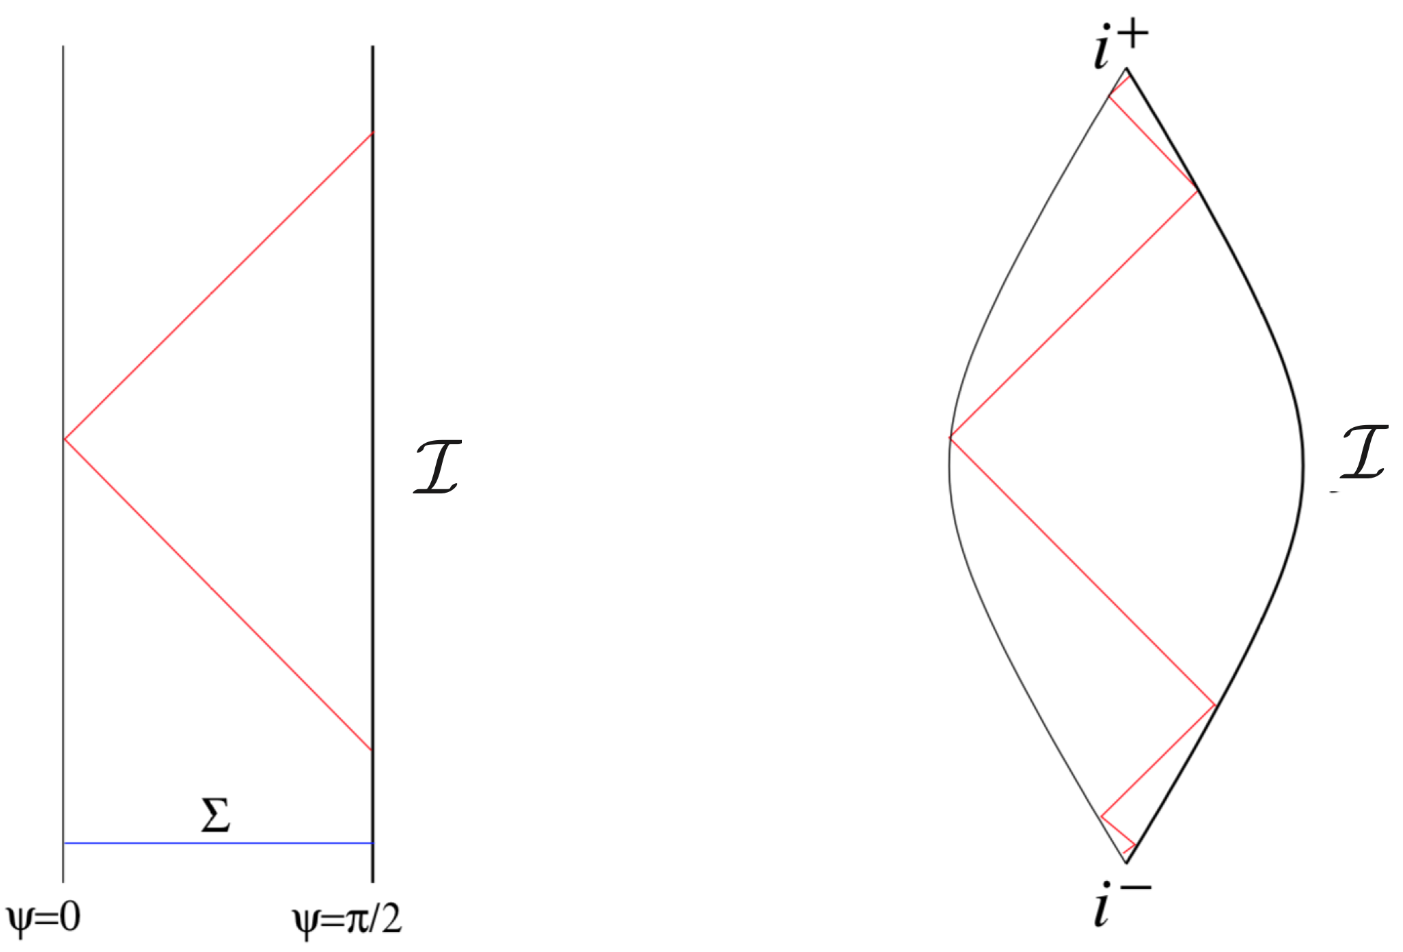
\includegraphics[width = 0.60 \textwidth]{ads-penr.png}
  \caption{Penrose diagrams for AdS, without and with conformally compactified time coordinate.}
  \label{ads-penr}
\end{figure}

\begin{proposition}
  AdS spacetime has a timelike $ \R \times \mathbb{S}^2 $ boundary with spacelike normal vector.
\end{proposition}

Note that $ \R $ is the time factor.\\
The Penrose diagram clearly shows that light rays reach the boundary in finite conformal time. To study physics in AdS, one needs to specify boundary conditions at $ \mathcal{I} $: for example, reflecting boundary conditions make light rays bounce back and forth forever, rendering AdS a $ \virgolette{box} $ spacetime in which massive particle are confined in the interior and massless particles bounce off the boundary.\\
Another characteristic of AdS space is that it isn't \textit{globally hyperbolic}: there exists no Cauchy surface on which initial data can be specified. Consider for example the 3d spacelike hypersurface $ \Sigma $ in Fig. \ref{ads-penr}. Specifying initial data on $ \Sigma $ it's not sufficient to solve for their time evolution: in AdS, there exist points in the future of $ \Sigma $ which are in causal contact with the boundary, thus the time evolution depends on boundary conditions too.\\
To make the Penrose diagram for AdS not stretch to infinity, the time coordinate can be restricted to finite values by:
\begin{equation*}
  \tilde{t} = \tan \tau
  \quad \Rightarrow \quad
  ds^2 = \frac{R^2}{\cos^2 \psi \, \cos^4 \tau} \left( -d\tau^2 + \cos^4 \tau \, d\Omega_3^2 \right)
\end{equation*}
This metric is conformally equivalent to:
\begin{equation*}
  d\tilde{s}^2 = - d\tau^2 + \cos^4 \tau \left( d\psi^2 + \sin^2 \psi \, d\Omega_2^2 \right)
\end{equation*}
with conformally compactified $ \tau \in \left[ - \frac{\pi}{2}, + \frac{\pi}{2} \right] $. Ignoring the spatial $ \mathbb{S}^2 $, the resulting Penrose diagram is drawn in Eq. \ref{ads-penr}: the spatial $ \mathbb{S}^3 $ grows and shrinks in time, the timelike boundary $ \mathcal{I} $ is still present and now the past and future timelike infinities $ i^{\pm} $ are also shown. This diagram makes it clear that a lightray bounces back and forth off teh boundary of AdS an infinite number of times.

\section{Matter coupling}

Spacetime is not merely the background on which matter exists, but it is dynamically influenced by the matter distribution on it. It is therefore necessary to study how matter couples to the spacetime metric.

\subsection{Field theories in curved spacetime}

The simplest way to describe matter is by fields governed by a Lagrangian. Consider a scalar field $ \phi(x) $. In flat Minkowski spacetime, its action is:
\begin{equation}
  \mathcal{S}_{\text{scalar}} \defeq \int d^4 x \left[ - \frac{1}{2} \eta^{\mu \nu} \pa_\mu \phi \pa_\nu \phi - V(\phi) \right]
  \label{eq:4.36}
\end{equation}
The negative sign of the kinetic term follows from the signature choice $ (-,+,+,+) $. The generalization to curved spacetime is straightforward:
\begin{equation*}
  \mathcal{S}_{\text{scalar}} = \int d^4 x \sqgm \left[ - \frac{1}{2} g^{\mu \nu} \na_\mu \phi \na_\nu \phi - V(\phi) \right]
\end{equation*}
Note the (useful) redundancy $ \na_\mu \phi = \pa_\mu \phi $. Curved spacetime also introduces the possibility to add new terms to the Lagrangian. For example:
\begin{equation}
  \mathcal{S}_{\text{scalar}} = \int d^4 x \sqgm \left[ - \frac{1}{2} \na_\mu \phi \na_\nu \phi - V(\phi) - \frac{1}{2} \xi R \phi^2 \right]
  \label{eq:4.37}
\end{equation}
for some $ \xi \in \R $. This theory correctly reduces to Eq. \ref{eq:4.36} on flat spacetime, as $ R = 0 $. To derive the equation of motion, vary the action keeping the metric fixed:
\begin{equation*}
  \begin{split}
    \delta \mathcal{S}_{\text{scalar}}
    &= \int d^4 x \sqgm \left[ - g^{\mu \nu} \na_\mu \delta \phi \na_\nu \phi - \frac{\pa V}{\pa \phi} \delta \phi - \xi R \phi \delta \phi \right] \\
    &= \int d^4 x \sqgm \left[ \left( g^{\mu \nu} \na_\mu \na_\nu \phi - \frac{\pa V}{\pa \phi} - \xi R \phi \right) \delta \phi - \na_\mu ( \delta \phi \na^\mu \phi ) \right]
  \end{split}
\end{equation*}
where integration by parts was possible due to $ \na_\mu g_{\rho \sigma} = 0 $ for the Levi-Civita connection. The last term is, by divergence theorem, a boundary term, thus the equation of motion for a scalar field theory in curved spacetime is:
\begin{equation}
  g^{\mu \nu} \na_\mu \na_\nu \phi - \frac{\pa V}{\pa \phi} - \xi R \phi = 0
  \label{eq:4.38}
\end{equation}
Now covariant derivatives are necessary, as $ \na_\mu \na_\nu \neq \pa_\mu \pa_\nu $.

\subsection{Einstein equations with matter}

To understand how matter fields back-react on spacetime, consider the combined action:
\begin{equation}
  \mathcal{S} = \frac{1}{16\pi G} \int d^4 x \sqgm \left( R - 2 \Lambda \right) + \mathcal{S}_M
  \label{eq:4.39}
\end{equation}
where $ \mathcal{S}_M $ is the action for matter fields, which in general depends on both the fields and the metric.

\begin{definition}\label{def-em-tens}
  Given a field theory for matter described by the action $ \mathcal{S}_M $, the \textit{energy-momentum tensor} is defined as:
  \begin{equation}
    T_{\mu \nu} \defeq - \frac{2}{\sqgm} \frac{\delta \mathcal{S}_M}{\delta g^{\mu \nu}}
    \label{eq:4.40}
  \end{equation}
\end{definition}

\begin{proposition}
  The energy-momentum tensor is symmetric.
\end{proposition}
\begin{proof}
  It inherits the symmetry of the metric.
\end{proof}

\begin{proposition}
  The equations of motion derived from the action Eq. \ref{eq:4.39} are:
  \begin{equation}
    G_{\mu \nu} + \Lambda g_{\mu \nu} = 8\pi G T_{\mu \nu}
    \label{eq:4.41}
  \end{equation}
\end{proposition}
\begin{proof}
  Varying the full metric, by Def. \ref{def-em-tens}:
  \begin{equation*}
    \delta \mathcal{S} = \frac{1}{16\pi G} \int d^4 x \sqgm \left[ G_{\mu \nu} + \Lambda g_{\mu \nu} \right] \delta g^{\mu \nu} - \frac{1}{2} \int d^4 x \sqgm T_{\mu \nu} \delta g^{\mu \nu} = 0
  \end{equation*}
\end{proof}

These are the full \textit{Einstein field equations}, describing gravity coupled to matter. It is possible to rewrite them by observing that the cosmological constant can be absorbed in the energy-momentum tensor as an additive component:
\begin{equation*}
  (T_\Lambda)_{\mu \nu} = - \frac{\Lambda}{8\pi G} g_{\mu \nu}
\end{equation*}
This is justified by the fact that matter fields often mimic a cosmological constant. Contracting the remaining equation with $ g^{\mu \nu} $ (i.e. taking the trace) then gives $ -R = 8\pi G T $, where $ T \equiv g^{\mu \nu} T_{\mu \nu} $, hence:
\begin{equation}
  R_{\mu \nu} = 8\pi G \left( T_{\mu \nu} - \frac{1}{2} T g_{\mu \nu} \right)
  \label{eq:4.42}
\end{equation}
Remember that the cosmological constant is present inside the energy-momentum tensor.

\subsection{Energy-momentum tensor}

The action $ \mathcal{S}_M $ is, by hypothesis, diffeomorphism-invariant, thus, recalling the argument which lead to Bianchi identity Eq. \ref{eq:4.13}, given $ \delta g_{\mu \nu} = (\ld_X g_{\mu \nu}) = 2 \na_{(\mu} X_{\nu)} $:
\begin{equation*}
  \delta \mathcal{S}_M = - \frac{1}{2} \int d^4 x \sqgm T_{\mu \nu} \delta g^{\mu \nu} = -2 \int d^4 x \sqgm T_{\mu \nu} \na^\mu X^\nu
\end{equation*}
Diffeomorphism invariance means that $ \delta \mathcal{S}_M = 0 $ for all $ X \in \xm $, hence, integrating by parts:
\begin{equation}
  \na_\mu T^{\mu \nu} = 0
  \label{eq:4.43}
\end{equation}
Of course, this was necessary to make Einstein equations consistent, as $ \na_\mu G^{\mu \nu} = 0 $. Anyway, this equation hints to the more profound nature of the energy-momentum tensor, which has nothing to do with gravity: it can be shown that the energy-momentum tensor is linked to Noether currents associated to translational invariance in space and time. Trivially, Eq. \ref{eq:4.43} reduces in flat spacetime to $ \pa_\mu T^{\mu \nu} = 0 $, which is the usual conservation law enjoyed by Noether currents.\\
Consider a translation $ x^\mu \mapsto x^\mu + \delta x^\mu $, with $ \delta x^\mu = X^\mu(x) $. The action restricted to flat spacetime is not invariant under such shift, but one which is invariant can be constructed coupling the matter fields to a background metric and allowing this to vary. The change of the action in flat space, where the metric is fixed, must be equal and opposite to the change of the action where the metric can vary but $ x^\mu $ is fixed, thus:
\begin{equation*}
  \begin{split}
    \delta \mathcal{S}_{\text{flat}}
    &= - \int d^4 x\, \frac{\delta \mathcal{S}_M}{\delta g^{\mu \nu}} \bigg\vert_{g_{\mu \nu} = \eta_{\mu \nu}} \delta g^{\mu \nu} = - \int d^4 x\, \frac{\delta \mathcal{S}_M}{\delta g^{\mu \nu}} \bigg\vert_{g_{\mu \nu} = \eta_{\mu \nu}} \pa^{(\mu} X^{\nu)} \\
    &= - 2 \int d^4 x\, \frac{\pa \mathcal{S}_M}{\pa g^{\mu \nu}} \bigg\vert_{g_{\mu \nu} = \eta_{\mu \nu}} \pa^\mu X^\nu = - 2 \int d^4 x\, \pa^\mu \left[ \frac{\pa \mathcal{S}_M}{\pa g^{\mu \nu}} \right]_{g_{\mu \nu} = \eta_{\mu \nu}} X^\nu
  \end{split}
\end{equation*}
But $ \delta \mathcal{S}_{\text{flat}} = 0 $ for all constant $ X^\mu $, as this is the definition of a translationally-invariant theory, hence the conserved Noether current in flat space is:
\begin{equation*}
  T_{\mu \nu} = - 2 \frac{\pa \mathcal{S}_M}{\pa \delta g^{\mu \nu}} \bigg\vert_{g_{\mu \nu} = \eta_{\mu \nu}}
\end{equation*}
i.e. the flat version of Eq. \ref{eq:4.40}.

\subsubsection{Field theories}

It is straightforward to compute $ T_{\mu \nu} $ for a scalar field $ \phi(x) $. Recall Eq. \ref{eq:4.37} (with $ \xi = 0 $) and Lemma \ref{lemma-sqgm}:
\begin{equation*}
  \delta \mathcal{S}_{\text{scalar}} = \int d^4 x \sqgm \left[ \frac{1}{4} g_{\mu \nu} \na^\rho \phi \na_\rho \phi + \frac{1}{2} g_{\mu \nu} V(\phi) - \frac{1}{2} \na_\mu \phi \na_\nu \phi \right] \delta g^{\mu \nu}
\end{equation*}
This gives the energy-momentum tensor:
\begin{equation}
  T_{\mu \nu} = \na_\mu \phi \na_\nu \phi - g_{\mu \nu} \left( \frac{1}{2} \pa^\rho \phi \na_\rho \phi + V(\phi) \right)
  \label{eq:4.44}
\end{equation}
Restricting to flat Minkowski spacetime:
\begin{equation*}
  T_{00} = \frac{1}{2} \dot{\phi}^2 + \frac{1}{2} (\na \phi)^2 + V(\phi)
\end{equation*}
which is the energy density of a scalar field.

\paragraph{Maxwell theory}

Varying Maxwell action Eq. \ref{eq:3.44}:
\begin{equation*}
  \delta \mathcal{S}_{\text{Maxwell}} = - \frac{1}{4} \int dx^4 \sqgm \left[ - \frac{1}{2} g_{\mu \nu} F^{\rho \sigma} F_{\rho \sigma} + 2 g^{\rho \sigma} F_{\mu \rho} F_{\nu \sigma} \right] \delta g^{\mu \nu}
\end{equation*}
So the energy-momentum tensor for Maxwell theory is:
\begin{equation}
  T_{\mu \nu} = g^{\rho \sigma} F_{\mu \rho} F_{\nu \sigma} - \frac{1}{4} g_{\mu \nu} F^{\rho \sigma} F_{\rho \sigma}
  \label{eq:4.45}
\end{equation}
In flat Minkowski spacetime:
\begin{equation*}
  T_{00} = \frac{1}{2} \ve{E}^2 + \frac{1}{2} \ve{B}^2
\end{equation*}
which is the energy density of the electromagnetic field.

\subsubsection{Perfect fluids}

A perfect fluid is described by its \textit{energy density} $ \rho(\ve{x},t) $, pressure $ p(\ve{x},t) $ and velocity 4-vector field $ u^\mu(\ve{x},t) : u^\mu u_\mu = -1 $. Pressure and energy density are related by an \textit{equation of state} $ p = p(\rho) $.

\begin{example}
  Dust is a fluid of massive particles floating around very slowly, so that the equation of state is $ p = 0 $.
\end{example}
\begin{example}
  Radiation is a fluid of photons with $ p = \rho / 3 $.
\end{example}

The energy-momentum tensor of a perfect fluid is:
\begin{equation}
  T^{\mu \nu} = (\rho + p) u^\mu u^\nu + p g^{\mu \nu}
  \label{eq:4.46}
\end{equation}
A fluid at rest ($ u^\mu = \delta_\mu,0 $) in flat Minkowski spacetime has $ T^{\mu \nu} = \diag \left( \rho, p, p, p \right) $, thus $ T_{00} $ is yet again the energy density, as expected. Generally, $ \rho = T_{\mu \nu} u^\mu u^\nu $ is the energy density measured by an observer co-moving with the fluid.\\
Bianchi identity $ \na_\mu T^{\mu \nu} = 0 $ determines two constraints. The first is:
\begin{equation}
  u^\mu \na_\mu \rho + (\rho + p) \na_\mu u^\mu = 0
  \label{eq:4.47}
\end{equation}
which is a generalization of mass conservation (where mass is identified with $ \rho $). The first term calculates how fast $ \rho $ changes along $ u^\mu $, while the second expresses it depending on the rate of flow out of the region $ \na_\mu u^\mu $. The second constraint is:
\begin{equation}
  (\rho + p) u^\mu \na_\mu u^\nu = - (g^{\mu \nu} + u^\mu u^\nu) \na_\mu p
  \label{eq:4.48}
\end{equation}
which is a generalization of Euler equation, i.e. the fluid equivalent of $ F = ma $ (or rather $ ma = F $).

\subsection{Energy conservation}

There's a difference between the energy-momentum tensor and the current which arises from a global symmetry. Consider a conserved current $ J^\mu : \na_\mu J^\mu = 0 $. Invoking the divergence theorem Eq. \ref{eq:3.41}:
\begin{equation*}
  0 = \int_V d^4 x \sqgm\, \na_\mu J^\mu = \int_{\pa V} d^3 x \sqrt{\gamma}\, n_{\mu} J^\mu
\end{equation*}
where $ V $ is a spatial volume with boundary $ \pa V = \Sigma_1 \cup \Sigma_2 \cup B $, with $ \Sigma_1, \Sigma_2 $ past and future spacelike boundarires and $ B $ timelike (lateral) boundary. If no current flows out of the region, i.e. $ n_\mu J^\mu \vert_B = 0 $, then this expression becomes the conservation $ Q(\Sigma_1) = Q(\Sigma)_2 $ of the charge associated to the current:
\begin{equation*}
  Q(\Sigma) \equiv \int_\Sigma d^3 x \sqrt{\gamma}\, n_\mu J^\mu
\end{equation*}
Thus, for a vector field, covariant conservation is equivalent to actual conservation.\\
The same argument doesn't apply to the energy-momentum tensor: the problem arises from generalizing $ \na_\mu J^\mu = \frac{1}{\sqgm} \pa_\mu (\sqgm J^\mu) $ to a higher-order tensor field, which is necessary in order to have a divergence theorem like Eq. \ref{eq:3.41}. Indeed:
\begin{equation*}
  \na_\mu T^{\mu \nu} = \pa_\mu T^{\mu \nu} + \Gamma^\mu_{\mu \rho} T^{\rho \nu} + \Gamma^\nu_{\mu \rho} T^{\mu \rho} = \frac{1}{\sqgm} \pa_\mu (\sqgm\, T^{\mu \nu}) + \Gamma^\nu_{\mu \rho} T^{\mu \rho}
\end{equation*}
The last term doesn't allow to convert the integral of $ \na_\mu T^{\mu \nu} $ to a boundary term. Instead:
\begin{equation}
  \pa_\mu (\sqgm\, T^{\mu \nu}) = -\sqgm\, \Gamma^\nu_{\mu \rho} T^{\mu \rho}
  \label{eq:4.49}
\end{equation}
Therefore, for higher-order tensors, covariant conservation is not equivalent to actual conservation.

\subsubsection{Conserved energy from Killing vectors}

Given a Killing vector $ K $, it's possible to define a conserved current associated to the energy-momentum tensor as:
\begin{equation}
  J_T^\nu \defeq - K_\mu T^{\mu \nu}
  \label{eq:4.50}
\end{equation}
This current is covariantly conserved, as:
\begin{equation*}
  \na_\nu J_T^\nu = - \left( T^{\mu \nu} \na_\nu K_\mu + K_\mu \na_\nu T^{\mu \nu} \right) = - T^{\mu \nu} \na_{(\nu} K_{\mu)} = 0
\end{equation*}
Its associated conserved charge on a spatial hypersurface $ \Sigma $ is defined as:
\begin{equation}
  Q_T(\Sigma) \defeq \int_\Sigma d^3 x \sqrt{\gamma}\, n_\mu J_T^\mu
  \label{eq:4.51}
\end{equation}
The interpretation of this charge depends on the properties of the Killing vector: if $ K $ is globally timelike, then the charge is the energy of matter $ E = Q_T(\Sigma) $, meanwhile if $ K $ is globally spacelike, then it is the momentum of matter.

\paragraph{Absence of Killing vectors}

The problem of energy conservation becomes subtle when dealing with spacetimes which do not have any globally timelike Killing vector.\\
For example, a system comprised of two orbiting stars is modelled by a spacetime which doesn't have such a Killing vector: however, the problem of matter energy conservation does not arise in this case, as the stars, while orbiting each other, emit gravitational waves, thus losing energy and eventually spiraling towards each other. Nonetheless, a meaningful question is that of energy conservation of the total system, i.e. the two stars and the gravitational field. A guess would be to consider a total energy-momentum tensor defined similarly to Eq. \ref{eq:4.40}, but:
\begin{equation*}
  T^{\text{total}}_{\mu \nu} = - \frac{2}{\sqgm} \left[ \frac{1}{16\pi G} \frac{\delta \mathcal{S}_{\text{EH}}}{\delta g^{\mu \nu}} + \frac{\delta \mathcal{S}_M}{\delta g^{\mu \nu}} \right] = - \frac{1}{8\pi G} G_{\mu \nu} + T_{\mu \nu} = 0
\end{equation*}
by Einstein field equations. This equation has no physical significance other than expressing the subtlety of energy conservation in Genera Relativity.\\
Clearly, one could try to understand the energy carried by the gravitational field alone. Unfortunately, there are compelling arguments that there exists no tensor which can be thought as the local energy density of the gravitational field: roughly speaking, the energy density of the Newtonian gravitational field $ \Phi $ is proportional to $ (\na \Phi)^2 $, so the relativistic equivalent should be proportional to the first derivatives of the metric, which can be made locally vanishing by normal coordinates due to the equivalence principle, and a tensor which vanishes in one coordinate system does so in all of them.










